\documentclass[aspectratio=169,11pt]{beamer}

% Shared style (ib-tutorials.sty at the repo root).
\makeatletter\def\input@path{{./}{../}}\makeatother
\usepackage{ib-tutorials}

\usepackage[utf8]{inputenc}
\usepackage{amsmath,amssymb}
\usepackage{booktabs}
\usepackage{array}
\newcolumntype{L}[1]{>{\raggedright\arraybackslash}p{#1}}
\usepackage{graphicx}
\graphicspath{{../pictures/5-visit/}{pictures/5-visit/}{../pictures/4-ibfe/}{pictures/4-ibfe/}}
\usepackage{xcolor}
\usepackage{listings}
\usepackage{tikz}
\usetikzlibrary{arrows.meta,positioning,shapes.geometric,fit,calc}
\usepackage{hyperref}

\newcommand{\sourcecredit}[1]{\vfill\begin{flushright}\tiny\textcolor{DarkGray}{#1}\end{flushright}}
\newcommand{\gui}[1]{\textsf{\textbf{#1}}}

\lstset{
  basicstyle=\ttfamily\scriptsize\color{BlackGray},
  keywordstyle=\color{NavyBlue}\bfseries,
  commentstyle=\color{DarkGray}\itshape,
  stringstyle=\color{OliveGreen},
  showstringspaces=false,
  columns=fullflexible,
  keepspaces=true,
  breaklines=true,
  breakindent=1em,
  frame=single,
  framerule=0.4pt,
  rulecolor=\color{LightGray},
  backgroundcolor=\color{LightGray!30},
  xleftmargin=0.25em,
  xrightmargin=0.25em
}
\lstdefinestyle{shell}{morecomment=[l]{\#}}
\lstdefinestyle{input}{morecomment=[l]{//}}
\lstdefinestyle{python}{morecomment=[l]{\#}}
\lstdefinestyle{cpp}{language=C++,morecomment=[l]{//}}
\lstdefinestyle{data}{}
\lstdefinestyle{tiny}{basicstyle=\ttfamily\tiny\color{BlackGray}}
\lstdefinestyle{inputtiny}{morecomment=[l]{//},basicstyle=\ttfamily\tiny\color{BlackGray}}
\lstdefinestyle{pytiny}{morecomment=[l]{\#},basicstyle=\ttfamily\tiny\color{BlackGray}}

\title[VisIt: Lagrangian and finite-element data]{VisIt: Lagrangian and finite-element data}
\subtitle{The Silo files of a point-method run and the ExodusII files of an IBFE run: what is in them, how to draw the structure where it is, colour it by its own fields, pick, select, query it over time, and get it out}
\author[Miller]{Laura A. Miller}
\institute[UArizona]{Department of Mathematics, University of Arizona}
\date{Using IB Software \textbullet\ Part V \textbullet\ Chapter 28}

\begin{document}

% 1
\begin{frame}[plain]
\maketutorialtitlepanel{%
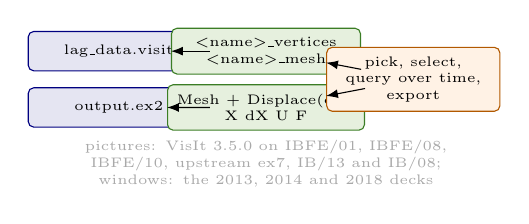
\begin{tikzpicture}[scale=0.55, every node/.style={font=\tiny}]
  \node[draw=NavyBlue,fill=NavyBlue!10,rounded corners=2pt,minimum width=2.3cm,minimum height=0.5cm] (a) at (0,0) {\code{lag\_data.visit}};
  \node[draw=NavyBlue,fill=NavyBlue!10,rounded corners=2pt,minimum width=2.3cm,minimum height=0.5cm] (b) at (0,-1.3) {\code{output.ex2}};
  \node[draw=OliveGreen,fill=OliveGreen!10,rounded corners=2pt,minimum width=2.4cm,minimum height=0.5cm,align=center] (m) at (3.4,0) {\code{<name>\_vertices}\\\code{<name>\_mesh}};
  \node[draw=OliveGreen,fill=OliveGreen!10,rounded corners=2pt,minimum width=2.4cm,minimum height=0.5cm,align=center] (p) at (3.4,-1.3) {\code{Mesh} + Displace(\code{dX})\\\code{X dX U F}};
  \node[draw=orange!70!black,fill=orange!10,rounded corners=2pt,minimum width=2.2cm,minimum height=0.5cm,align=center] (f) at (6.8,-0.65) {pick, select,\\query over time,\\export};
  \draw[-{Latex[length=1.5mm]}] (a) -- (m); \draw[-{Latex[length=1.5mm]}] (b) -- (p);
  \draw[-{Latex[length=1.5mm]}] (m) -- (f); \draw[-{Latex[length=1.5mm]}] (p) -- (f);
  \node[text=DarkGray,align=center,text width=5.6cm] at (3.4,-2.6) {pictures: VisIt 3.5.0 on IBFE/01, IBFE/08, IBFE/10, upstream ex7, IB/13 and IB/08; windows: the 2013, 2014 and 2018 decks};
\end{tikzpicture}}
\end{frame}

% 2
\begin{frame}{Learning goals}
\label{fr:goals}
\footnotesize By the end of this chapter you should be able to:
\begin{enumerate}
  \item say what a point-method run writes for VisIt about its structure (the Silo files behind \code{lag\_data.visit}: positions only, as \code{<name>\_vertices} and \code{<name>\_mesh}) and what an IBFE run writes (one ExodusII file per part with the reference mesh and the nodal fields \code{X}, \code{dX}, \code{U}, \code{F});
  \item draw a finite-element mesh where it is now (the Displace operator with the displacement \code{dX}), on top of the fluid, for one part, several parts, and in 3D;
  \item colour the mesh by its own fields and by expressions of them, draw its velocity as vectors, and judge its element quality with VisIt's \code{mesh\_quality} expressions;
  \item read numbers off the structure: Pick a node, query the maximum, minimum or average of a field over the mesh or over a selected part of it, and plot that quantity against time;
  \item build the displacement of an IB point set from its positions when there is no \code{dX}, with a cross-time expression;
  \item export a mesh with its fields to VTK and a time query to a \code{.curve} file, and know which chapter reads them next (29, 32, 33).
\end{enumerate}
\begin{punchbox}
\scriptsize The plot pictures are new (VisIt 3.5.0 headless on this series' runs; \code{wsl/final/visit\_ch28.sh}); the window screenshots come from the 2013, 2014 and 2018 decks (VisIt 2.x on a Mac) and are credited on each slide; the 3.x names are in the text. Everything stated about the files was checked against the IBAMR 0.19.0 source and VisIt's own metadata of the files.
\end{punchbox}
\end{frame}

% 3
\begin{frame}{Where this chapter comes from}
\label{fr:sources}
\scriptsize
\begin{itemize}
  \item \al{``IBAMR Finite Element Visualization in VisIt'' (Alex Hoover, Miller Lab, 23 May 2013; a Word document, and a 7-slide deck titled ``\ldots with VisIt''):} the recipe every later version repeats: open \code{dumps.visit} and \code{output.ex2}, untick \gui{Apply operators to all plots}, Mesh plot, \gui{Operators $\to$ Transforms $\to$ Displace}, create the vector expression \code{dX}, save it as XML, Project for the old 2D-in-3D output, and the examples list. Re-issued on the Drive as ``0-IBFE Tutorial: Visualizing FE boundaries with VisIt'' (the document, 2017; the slides, edited to 2024), as deck 3 of the 2018--19 Visualization and Data Analysis series, as ``Lecture 3'' of the 2020 visualization series, and as slides 18--26 of the 2020/2024 IBFE Lecture 1 (chapter 17 describes that deck).
  \item \al{``5-IBFE Tutorial: Visualizing Lagrangian Data'' (Hoover, 2014; 9 slides, VisIt 2.7.2):} the fields in the Exodus file, query over time, selection, expressions, on a 3D jellyfish-bell ring; its nine screenshots are reused.
  \item \al{``3B -- Analyzing your IBFE simulation'' (MATH 769, 2018; 16 slides, VisIt 2.12.3 on KillDevil):} recording the GUI to Python, exporting \code{.ex2} as VTK for a cluster whose VisIt could not read Exodus, the Box average over time, the \code{.curve} file and its MATLAB import. The recording part is chapter 32; the Eulerian box average chapter 29; the Lagrangian export and the curve file are here.
  \item \al{MATH 769 ``IBAMR with FE'' (April 2013), slides 9--10:} Boyce Griffith's description of the file from the IBAMR mailing list, quoted on slide \ref{fr:griffith}.
  \item \al{New here:} the Silo writer read from the source (\code{LSiloDataWriter.cpp}, \code{IBRedundantInitializer.cpp}): the file layout, the names, what is and is not written; VisIt 3.5's metadata of each file (the vector expressions it now builds itself; \code{mesh\_quality}); the Pick output; the domain Subset; a cross-time displacement for IB points; the error texts; the 3D and multi-part cases on this series' runs; the exported files shown as they come out.
\end{itemize}
\end{frame}

% 4
\begin{frame}{Two kinds of Lagrangian output}
\label{fr:kinds}
\footnotesize
\begin{tabular}{@{}L{0.17\textwidth}L{0.30\textwidth}L{0.45\textwidth}@{}}
\toprule
method & files for VisIt & what they hold \\
\midrule
IB (points, springs, beams; Parts II--III) & \code{viz\_IB2d/lag\_data.visit} and the \code{lag\_data.cycle\_NNNNNN/} folders (Silo) & the positions of every point at every visualization dump, as a point mesh and as the edges of the springs; no velocity, no force (slide \ref{fr:silo2}) \\
IBFE (finite elements; Part IV) & \code{viz\_IB2d/output.ex2}, one ExodusII file per part (\code{beam\_output.ex2}, \code{circle\_output.ex2}, \ldots) & the reference mesh and, at every dump, the nodal fields: position \code{X}, displacement \code{dX}, velocity \code{U}, force density \code{F} (slide \ref{fr:exodus}) \\
ConstraintIB (chapter 14) & the same Silo files for the points & the kinematics, forces and energies are text files in \code{PrintOutput/} \\
IB2d (Part II) & \code{viz\_IB2d/lagsPts.NNNN.vtk} (and \code{lagsPtsConnect} when asked) & the points as VTK; chapter 26 drew them \\
\bottomrule
\end{tabular}

\begin{itemize}
  \item The forces and velocities of a point-method run are \emph{not} in its VisIt files: they are the \code{hier\_data} text files of chapter 11 (\code{X.*}, \code{F.*}), or the sums the program prints. VisIt shows where the points are.
  \item An IBFE run has the opposite arrangement: everything about the structure is in the Exodus file, and there is no \code{lag\_data.visit}.
  \item Both kinds sit next to the fluid's \code{dumps.visit} (chapter 26) and are opened as a second source in the same window.
\end{itemize}
\end{frame}

% 5
\begin{frame}[fragile]{The Silo files on disk}
\label{fr:silo1}
\footnotesize
\begin{columns}[T]
\column{0.5\textwidth}
\begin{lstlisting}[style=tiny]
viz_IB2d/                       # IB/13 human, 4 ranks
  dumps.visit                   # fluid (ch. 26)
  lag_data.visit                # 102 lines: one folder per frame
  lag_data.cycle_000000/
  lag_data.cycle_000341/
    lag_data.cycle_000341.summary.silo   # 2.8 kB
    lag_data.proc_0000.silo              # 30 kB
    lag_data.proc_0001.silo              # 1 kB
    lag_data.proc_0002.silo
    lag_data.proc_0003.silo
  lag_data.cycle_000682/ ...
\end{lstlisting}
\begin{lstlisting}[style=inputtiny]
Main {                       // what controls them
   viz_writer = "VisIt","Silo"   // "Silo" switches the writer on
   viz_dump_interval = 341
   viz_dump_dirname = "viz_IB2d"
}
\end{lstlisting}
\column{0.48\textwidth}
\scriptsize
\begin{itemize}
  \item The names are fixed in \code{LSiloDataWriter.cpp}: \code{lag\_data.visit}, the folder prefix \code{lag\_data.cycle\_}, the summary file \code{<folder>.summary.silo}, one \code{lag\_data.proc\_PPPP.silo} per MPI rank. The folder number is the time step, not the frame number.
  \item Each rank writes its own file; the summary file (written by rank 0) is a Silo \emph{multimesh} that lists them, and that is what \code{lag\_data.visit} points at. Open the \code{.visit} file; never a \code{proc} file.
  \item Why rank 0's file is big and the others are small: the initializer registers every structure on rank 0 (slide \ref{fr:silo2}), and the writer gathers that structure's points to the rank that registered it (a \code{VecScatter} from the owning ranks) before writing. The other ranks' files are empty Silo files (a root directory and nothing else; 1 kB each here). The points still live on the ranks that own their patches during the run.
\end{itemize}
\end{columns}
\end{frame}

% 5b
\begin{frame}{Who writes the Silo files, and what switches them on}
\label{fr:silo1b}
\footnotesize
\begin{itemize}
  \item Without \code{"Silo"} in \code{viz\_writer} no Lagrangian file is written; an IB/01-style program then also segfaults at its first dump (chapter 16's silent-failures table), because \code{getLSiloDataWriter()} returns null and the program dereferences it.
  \item The writer is created and registered in the program: \code{silo\_data\_writer = app\_initializer->getLSiloDataWriter()} and \code{ib\_method\_ops->registerLSiloDataWriter(silo\_data\_writer)} (every example's \code{main.cpp}; chapter 11 lists the outputs). The \code{LDataManager} then hands it the coordinates of every level (\code{registerCoordsData}) and the Lagrangian ordering (\code{registerLagrangianAO}); the initializer tells it which index ranges are structures and which edges are springs (next slide).
  \item The writer's own API could add fields to the points, \code{registerVariableData(name, LData, level)}, but \code{IBMethod} never calls it: a custom program can (chapter 11's output hooks are the place), and \code{GeneralizedIBMethod}, \code{IMPMethod}, \code{PenaltyIBMethod} (\code{Y}, \code{M}) and \code{CIBMethod} (\code{lambda}) do (slide \ref{fr:silo2b}).
\end{itemize}
\end{frame}

% 5c
\begin{frame}{When the Silo files are written, and what a restart keeps}
\label{fr:silo1c}
\footnotesize
\begin{itemize}
  \item \code{silo\_data\_writer->writePlotData(iteration\_num, loop\_time)} is called by the program's main loop (\code{main.cpp}), in the same \code{if} block as the fluid writer's \code{visit\_data\_writer->writePlotData(...)}, at every \code{viz\_dump\_interval} and at the last step; no integrator calls it. That is why the two time series have the same frames.
  \item The restart files hold the writer's registrations (structure names, index ranges, edge maps: \code{putToDatabase}), which is why the initializer does not re-register them after a restart. The folder numbers continue because they are the iteration numbers the program passes; \code{lag\_data.visit} itself is truncated at the first post-restart dump, so chapter 3's rebuild recipe applies to it as to \code{dumps.visit}.
  \item A frame is therefore the pair (SAMRAI dump, Silo dump) at one iteration; \code{viz\_dump\_interval} in \code{Main} is the only cadence, and \code{data\_dump\_interval} (the \code{hier\_data} text files of chapter 11) is independent of it.
\end{itemize}
\end{frame}

% 6
\begin{frame}{What is inside: names and contents}
\label{fr:silo2}
\scriptsize
\begin{tabular}{@{}L{0.26\textwidth}L{0.66\textwidth}@{}}
\toprule
Silo object & what it is (from \code{IBRedundantInitializer::initializeLSiloDataWriter}) \\
\midrule
\code{<structure>\_vertices} & a \emph{marker cloud}: the points of one structure file (\code{<structure>.vertex}), a 0-dimensional point mesh; registered for every structure \\
\code{<structure>\_mesh} & an \emph{unstructured mesh} whose edges are the springs of \code{<structure>.spring}; registered only when the structure has springs; the Mesh plot of it with a line width is the connected boundary of chapter 26 \\
\code{<structure>\_xmesh} & the same for the cross-links of a \code{.xspring} file \\
\code{<structure>\_rod\_mesh} & the rods of a \code{.rod} file; named \code{\_mesh} instead when no structure on that level registered a spring mesh (the flag is per level, not per structure) \\
beams, targets, anchors, masses & not drawn: no edge map is registered for them; a beam-only structure shows as points \\
\code{level\_L\_cloud\_K}, \code{level\_L\_mesh\_K} & the directories inside each \code{proc} file (one per level, cloud or mesh); the summary's multimesh gathers them under the structure's name \\
\code{domains}, \code{blocks} & the Subset categories VisIt makes from the multimesh: one domain per registered mesh (so one, \code{domain1}, for a structure registered on rank 0), not one per rank \\
\bottomrule
\end{tabular}
\end{frame}

% 6b
\begin{frame}{What is written for the points: variables, ranks, order}
\label{fr:silo2b}
\footnotesize
\begin{itemize}
  \item \al{Variables:} \code{LDataManager} registers the coordinates (\code{registerCoordsData}) and nothing else for \code{IBMethod}; VisIt's metadata of \code{lag\_data.visit} lists no scalars and no vectors. \code{GeneralizedIBMethod} adds the directors \code{D1}, \code{D2}, \code{D3} and the angular velocity \code{W}; \code{IMPMethod} adds \code{F0}--\code{F2} and \code{tau0}--\code{tau2}; \code{PenaltyIBMethod} (chapter 13) adds \code{Y} and \code{M}, \code{CIBMethod} \code{lambda}. So ``colour the points by their force'' is not possible from these files for the plain IB method: chapter 11's \code{hier\_data} files are the route, or a cross-time expression for the displacement (slide \ref{fr:cmfe}).
  \item \al{Who registers:} the initializer does it on MPI rank 0 only (``this will fail if the structure is too large to be stored in the memory available to a single MPI process'', the source's own warning); the names are the structure's base file name plus the postfix.
  \item \al{Order:} the writer keeps the Lagrangian numbering through the application ordering it is handed (\code{registerLagrangianAO}), so node $k$ of a frame is the point of line $k+2$ of the \code{.vertex} file (line 1 is the count) at every frame (checked on slide \ref{fr:pickpts}).
\end{itemize}
\end{frame}

% 7
\begin{frame}{VisIt's view of \code{lag\_data.visit}}
\label{fr:domains}
\footnotesize
\begin{columns}[T]
\column{0.44\textwidth}
\begin{center}
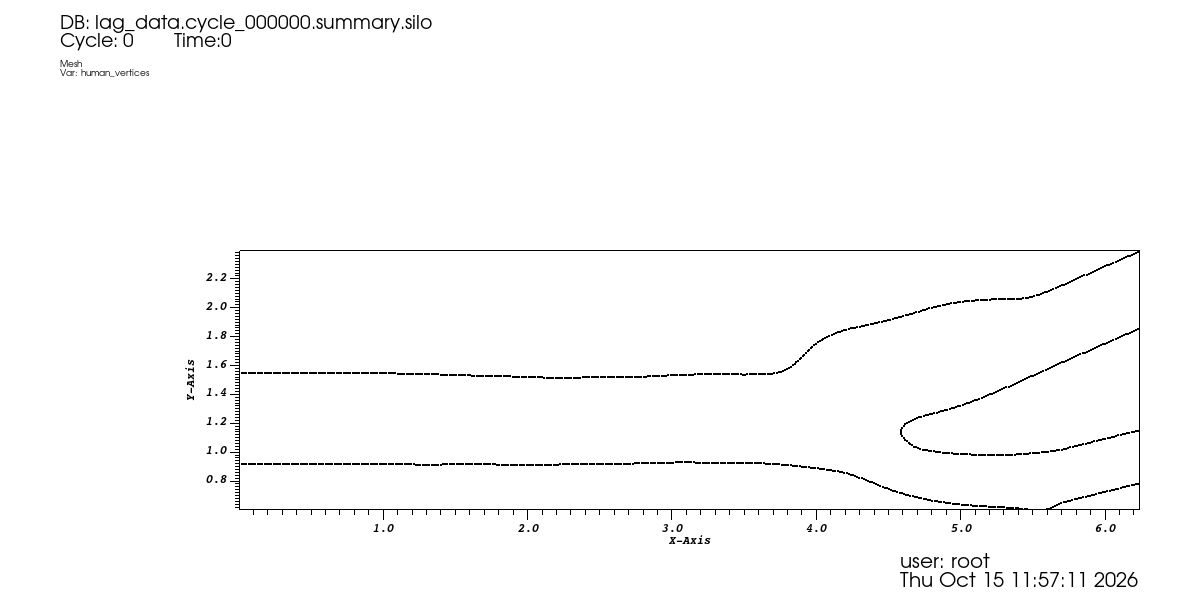
\includegraphics[width=0.49\textwidth]{ch26-1-points-default.png}\hfill
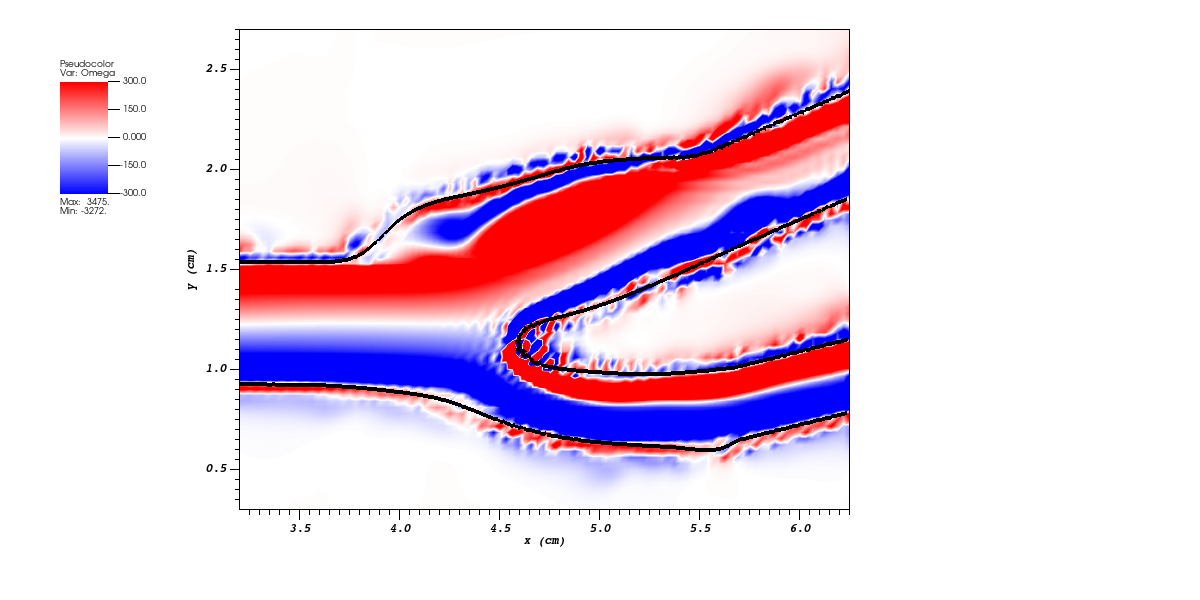
\includegraphics[width=0.49\textwidth]{ch26-8-mesh-edges.png}
\end{center}
\scriptsize IB/13 human (chapter 26): the Mesh plot of \code{human\_vertices} (points) and of \code{human\_mesh} (the spring edges, line width 3).
\column{0.54\textwidth}
\scriptsize
\begin{itemize}
  \item Metadata (\gui{File $\to$ File information}, or \code{GetMetaData} in the CLI): meshes \code{human\_mesh} and \code{human\_vertices}, 102 states with their times, one block each (block title \code{domains}, group title \code{blocks}), no scalars, no vectors, and the \code{mesh\_quality} expressions VisIt offers for any mesh.
  \item \gui{Add $\to$ Mesh} draws either (chapter 26). \gui{Add $\to$ Subset $\to$ domains} exists but colours everything alike: the structure was registered on one rank and is one domain (\code{domain1}); a run with two structure files has two meshes, not two domains.
  \item What is \emph{not} there: no velocity, no force, no displacement. The \code{time\_derivative} expressions VisIt lists for a mesh (\code{time(human\_vertices)}, \code{conn\_cmfe(...)}) are the building blocks of slide \ref{fr:cmfe}.
  \item A structure whose file has beams but no springs shows as points only; add a \code{.spring} file with zero stiffness if you want the edges drawn (chapter 6's format; stiffness 0 changes nothing in the run).
\end{itemize}
\end{columns}
\end{frame}

% 8
\begin{frame}[fragile]{Picking a point: node number = Lagrangian index}
\label{fr:pickpts}
\footnotesize
\begin{columns}[T]
\column{0.5\textwidth}
\begin{lstlisting}[style=tiny]
# CLI: PickByNode(domain=0, element=0) on human_vertices, frame 0 (positionally the node comes FIRST: PickByNode(node, domain))
A:  lag_data.cycle_000000.summary.silo  timestep 0
human_vertices
Point: <0.0078125, 0.920573>
Node:  0
Incident Zones:  0
\end{lstlisting}
\begin{lstlisting}[style=tiny]
# human.vertex, the structure file (chapter 6)
1045
7.8125000000000000e-03 9.2057340405399213e-01   # line 2 = node 0
2.3447577247806096e-02 9.2050862810363454e-01   # line 3 = node 1
\end{lstlisting}
\column{0.48\textwidth}
\scriptsize
\begin{itemize}
  \item In the GUI: \gui{Controls $\to$ Pick}, \gui{Node} mode, click a point; the Pick window prints its coordinates and node number, and a letter appears at the point. On a point mesh every point is also a one-node zone, so a Zone pick returns the same point (zone $k$ = node $k$).
  \item The node number is the Lagrangian index within the structure (0-based; the \code{.vertex} file's line $k + 2$), the same number \code{getNodeDataItem} (chapter 9a) and the \code{X.*} files of chapter 11 use. Two structures in one run (\code{human} and a second file) have separate meshes and separate numberings.
  \item \gui{Do time curve} in the Pick window turns the next pick into the history of that node: one curve per coordinate in window 2 (\gui{Multiple Y axes} or one). This is the quickest ``where did point 512 go'' tool; the scripted version (\code{PickByNode} in a loop over states) is chapter 32.
  \item \code{NumNodes} on the point mesh gives $1045$, the file's first line; the 2D Silo picture needs nothing else: the Pick confirms that node $0$ is the file's first point, $(0.0078125, 0.920573)$.
\end{itemize}
\end{columns}
\end{frame}

% 9
\begin{frame}[fragile]{A displacement for IB points: the cross-time expression}
\label{fr:cmfe}
\footnotesize
\begin{columns}[T]
\column{0.5\textwidth}
\begin{lstlisting}[style=tiny]
# Controls > Expressions (three of them, in this order)
pos       vector  coords(human_vertices)
pos0      vector  conn_cmfe(<[0]i:pos>, human_vertices)
disp_mag  scalar  magnitude(pos - pos0)
\end{lstlisting}
\begin{center}
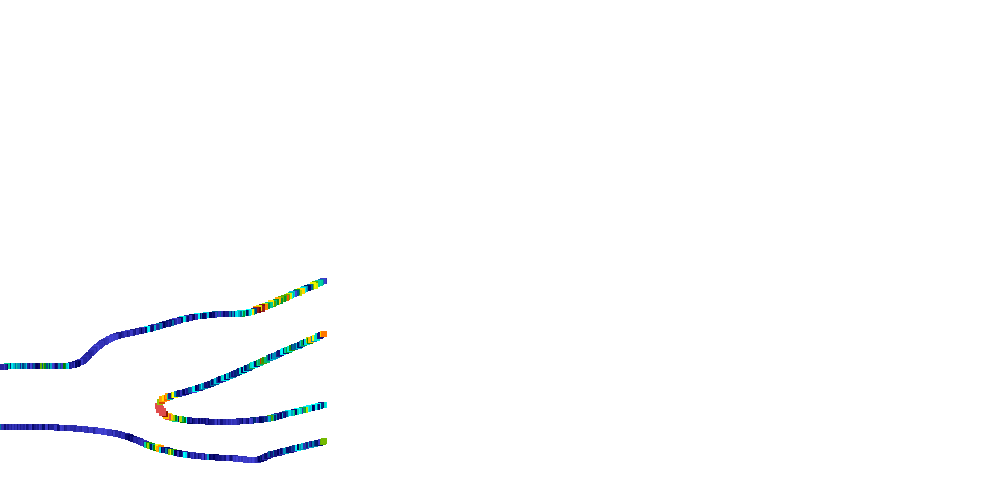
\includegraphics[width=0.8\textwidth]{ch28-silo-disp.png}
\end{center}
\column{0.48\textwidth}
\scriptsize
\begin{itemize}
  \item \code{coords(mesh)} is the position of each node as a vector; \code{conn\_cmfe(<[0]i:var>, mesh)} fetches \code{var} from state 0 (\code{[0]i} = absolute index 0; \code{[-1]id} would be the previous state) and maps it node by node, which is right because the writer keeps the numbering (slide \ref{fr:silo2}). The difference is the displacement since the first frame; its magnitude is a scalar to colour the points by.
  \item Picture: IB/13 human at frame 56; the displacement since $t = 0$ runs from $3\times10^{-5}$ to $0.029$ cm (its mean is well under a cell: the walls are target points), largest at the open ends where the outlet bands pull. The target points of this example barely move, which is the point of the picture: the expression measures how far the walls drift from their targets (chapter 9a's question).
\end{itemize}
\end{columns}
\end{frame}

% 9b
\begin{frame}[fragile]{The cross-time expression: variants}
\label{fr:cmfe2}
\footnotesize
\begin{lstlisting}[style=tiny]
pos_prev  vector  conn_cmfe(<[-1]id:pos>, human_vertices)   # the previous frame ([-1]id = relative index)
step_mag  scalar  magnitude(pos - pos_prev)                 # displacement per frame
speed_est scalar  magnitude(pos - pos_prev) / 0.01705       # divided by the frame interval: a velocity estimate
pos_t1    vector  conn_cmfe(<[56]i:pos>, human_vertices)    # any absolute frame, here the systolic peak
\end{lstlisting}
\begin{itemize}
  \item The same three lines with \code{[-1]id} give the displacement per frame, and divided by the frame interval, a velocity estimate at the dump cadence (coarse: $0.017$ s here, against the run's $5 \times 10^{-5}$ s step); the \code{X.*} files of chapter 11 give the exact velocity at the data-dump cadence instead.
  \item \code{conn\_cmfe} maps by connectivity (node $k$ to node $k$) and needs the same number of points in both frames, which a point-method run guarantees; \code{pos\_cmfe(<[0]i:var>, mesh, fill)} maps by position and is for meshes that change, or for sampling the fluid onto the structure (chapter 29).
  \item Expressions live in the session, not in the data: save the session (chapter 26) and \gui{Restore session with sources} on the next run; or keep them in a script (\code{DefineVectorExpression}, chapter 32).
  \item The GUI's \gui{Controls $\to$ Expressions} window has a \gui{Time iteration} tab for the same thing (``this variable at another time''); the typed form above is the one that scripts and sessions store.
\end{itemize}
\end{frame}

% 10
\begin{frame}{A 3D point cloud: IB/08 glycocalyx}
\label{fr:silo3d}
\footnotesize
\begin{columns}[T]
\column{0.5\textwidth}
\begin{center}
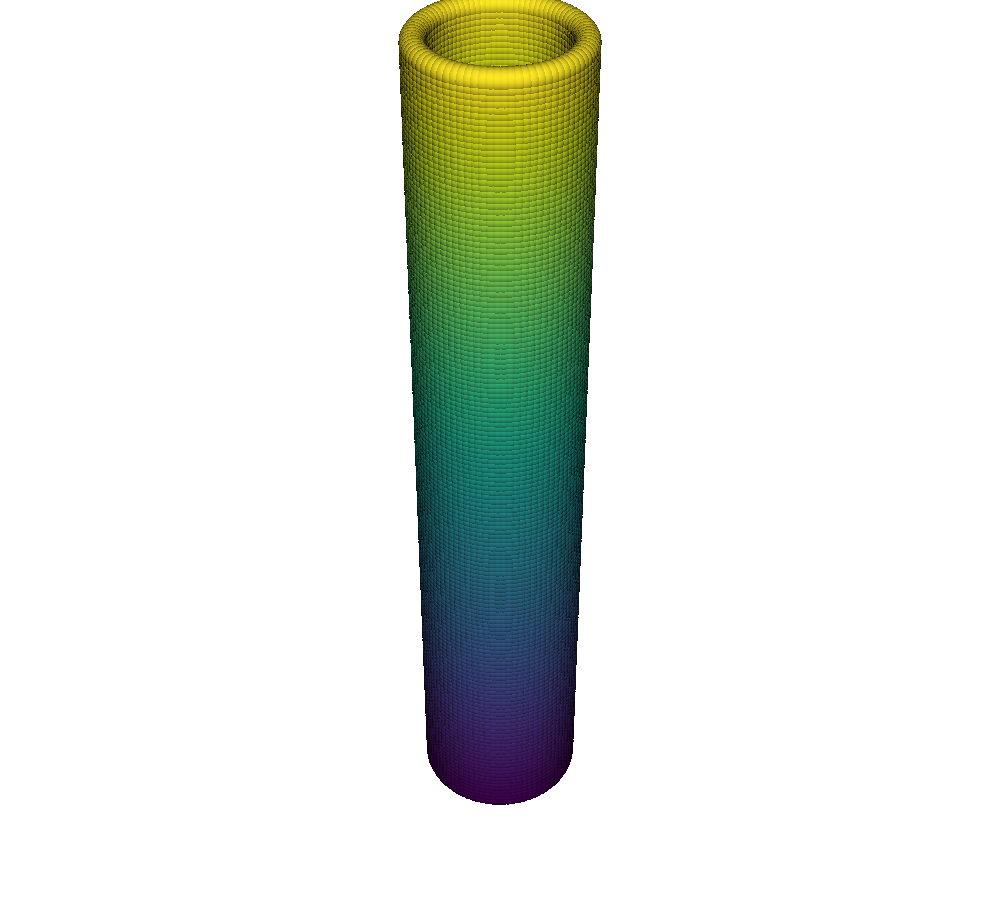
\includegraphics[width=0.6\textwidth]{ch28-silo-3d.png}
\end{center}
\scriptsize \code{glyco\_512\_vertices} as spheres coloured by height (\code{coords(glyco\_512\_vertices)[2]}) at $t = 0.2$: a hollow cylinder of points standing on the floor of the box.
\column{0.48\textwidth}
\scriptsize
\begin{itemize}
  \item A 3D run writes the same files into \code{viz\_IB3d/}; the cloud is a 3D point mesh. This structure has no springs (target points only), so there is no \code{\_mesh}: the Mesh plot of \code{glyco\_512\_mesh} that chapter 12's table named does not exist (``An invalid variable (glyco\_512\_mesh) was specified'').
  \item Points in 3D are invisible at the default size: in the Pseudocolor or Mesh attributes set \gui{Point type} to \gui{Sphere} and a \gui{Point size} in data units (or pixels); the Mesh plot has the same controls.
  \item Camera, slices and the 3D view are chapter 27; everything else on these slides (pick, subset, expressions, queries) works unchanged in 3D.
  \item The glycocalyx of IB/08 is target points without springs, so the file has \code{glyco\_512\_vertices} and no \code{\_mesh}: $13\,600$ points on a cylinder $0.026$ across and $0.156$ tall at the bottom of a box $1$ high. VisIt's \code{ResetView} frames the plots that exist, so draw the points first and add the fluid afterwards when the structure is a small part of the box.
\end{itemize}
\end{columns}
\end{frame}

% 11
\begin{frame}{The ExodusII file: what libMesh writes for IBFE}
\label{fr:exodus}
\scriptsize
\begin{tabular}{@{}L{0.24\textwidth}L{0.22\textwidth}L{0.46\textwidth}@{}}
\toprule
system (\code{FEMechanicsBase.cpp}) & variables & meaning \\
\midrule
\code{IB coordinates system} & \code{X\_0}, \code{X\_1} (\code{, X\_2}) & the current position of each node \\
\code{IB coordinate mapping system} & \code{dX\_0}, \code{dX\_1} (\code{, dX\_2}) & the displacement from the reference configuration, $\mathbf{X} - \mathbf{s}$: what the Displace operator wants \\
\code{IB velocity system} & \code{U\_0}, \code{U\_1} (\code{, U\_2}) & the node's velocity, interpolated from the fluid (``the velocity exerted on the mesh'' of the 2014 deck) \\
\code{IB force system} & \code{F\_0}, \code{F\_1} (\code{, F\_2}) & the Lagrangian force density (stress divergence, tethers, body forces) \\
\code{IB pressure system} & \code{P}, or \code{Phi} & \code{P} with a static or dynamic pressure part (\code{FEMechanicsBase}); \code{Phi} with \code{IBFEMethod}'s stress-normalization part (upstream ex0 uses it), written under the same system name; neither in this series' runs \\
\code{IB source system} & \code{Q} & a Lagrangian body source (\code{registerLagBodySourceFunction}); not in this series' runs \\
\bottomrule
\end{tabular}

\begin{itemize}
  \item \code{exodus\_io->write\_timestep(filename, *equation\_systems, n, time)} writes \emph{every} system's variables as nodal fields, one state per visualization dump numbered from 1 (chapter 17 showed the call and \code{exodus\_io->append(from\_restart)}, which continues the file after a restart instead of starting it over).
\end{itemize}
\end{frame}

% 11b
\begin{frame}{The ExodusII file (2): the mesh, the parts, and what switches it on}
\label{fr:exodus2}
\footnotesize
\begin{itemize}
  \item The mesh itself is written once, in its reference configuration, with its element blocks (the mesher's physical groups or Exodus blocks of chapter 18: one block \code{0} for the plate), node sets and side sets (upstream ex7's walls carry node sets).
  \item One file per part (chapter 21): \code{getExodusIIFilename("beam\_")} gives \code{viz\_IB2d/beam\_output.ex2}. The file is written by rank 0 from the gathered mesh, so it is one file whatever the rank count.
  \item \code{viz\_writer = "VisIt","ExodusII"} is what the examples write, but in 0.19.0 the second word is inert: \code{AppInitializer} starts with \code{d\_exodus\_filename = "output.ex2"} and \code{getExodusIIFilename()} returns it whether or not \code{"ExodusII"} is listed (the entry only lets an \code{exodus\_filename} key rename the file). The plate file is written whenever visualization dumps are on (\code{viz\_dump\_interval > 0}) and the program calls \code{write\_timestep}; a test run with \code{viz\_writer = "VisIt"} alone wrote \code{output.ex2}. Chapter 17's ``both words or no plate file'' is corrected with this chapter.
\end{itemize}
\end{frame}

% 12
\begin{frame}{Boyce Griffith on the file (2013)}
\label{fr:griffith}
\footnotesize
\begin{quote}
\scriptsize ``At present, with the IBFE examples, there is a file created in the viz directory named \code{output.ex2}. This is an ExodusII file. The file stores the reference configuration of the mesh (which need not be the initial configuration) as well as field data defined on the mesh, including the Lagrangian velocity field and force density. I do not know how to setup these files so that VisIt automatically recognizes that the individual components of a field belong to a vector field variable. If you want to visualize vector fields on the mesh, you have to set up a vector expression. E.g., you may wish to set up a vector expression \code{U} as \code{\{U\_0, U\_1, U\_2\}} (in 3D) or \code{\{U\_0, U\_1, 0\}} (in 2D). If you want to visualize the current configuration of the mesh, you need to set up a vector expression \code{dX = \{dX\_0, dX\_1, dX\_2\}} for the displacement between the reference and current configurations. You can then apply the `displace' operator to the mesh. Currently, 2D output is really stored in 3D, but with a trivial z component. If you want to simultaneously visualize 2D Eulerian and 2D FE data, you will need to apply the `project' operator to the FE data. Note that you will need to unselect `Apply operators to all plots' to prevent the displace and project operators from being applied to the Eulerian data.''
\end{quote}
\begin{itemize}
  \item Quoted without attribution in the MATH 769 deck of April 2013; by its content and its first-person voice it is Boyce Griffith's, presumably from the IBAMR users' list (the post itself was not found). Three things have changed since, and the next slide shows them in VisIt's own metadata: the vector expressions are built by VisIt now, 2D output is two-dimensional, and the Project step is gone. The rest is still exactly right.
\end{itemize}
\sourcecredit{MATH769\_IBFE.pptx (2013), slides 9--10; text attributed to B. Griffith.}
\end{frame}

% 13
\begin{frame}[fragile]{VisIt's view of \code{output.ex2} (IBFE/01, 3.5.0)}
\label{fr:meta}
\footnotesize
\begin{columns}[T]
\column{0.54\textwidth}
\begin{lstlisting}[style=tiny]
states 41, times 0.0, 0.1, ... 4.0
mesh    Mesh   spatial dim 2, topological dim 2, 1 block
scalars ElementBlock (zonal)
        F_0 F_1  U_0 U_1  X_0 X_1  dX_0 dX_1   (nodal)
        coordx coordy  node_num_map  elem_num_map
vectors (none in the file)
expressions, made by VisIt on opening:
        F  = {F_0, F_1}     U  = {U_0, U_1}
        X  = {X_0, X_1}     dX = {dX_0, dX_1}
        mesh_quality/area, aspect, condition, degree, jacobian,
        max_edge_length, maximum_angle, min_edge_length,
        min_corner_area, min_sin_corner, minimum_angle, oddy,
        relative_size, scaled_jacobian, shape, shear, skew, ...
NumNodes 101, NumZones 130
\end{lstlisting}
\column{0.44\textwidth}
\scriptsize
\begin{itemize}
  \item The Exodus reader of VisIt 3.5 groups variables named \code{name\_0}, \code{name\_1} into a vector expression \code{name} by itself in the 2D files (not in the 3D file: slide \ref{fr:threed}): \code{dX} is already under \gui{Vectors} in the Displace window, as the 2024 edit of the deck noticed (``for newer IBAMR versions, there should be a dX option under Vectors''). Creating it by hand (slide \ref{fr:recipe}) still works and does no harm.
  \item \code{coordx}, \code{coordy} are the reference coordinates as scalars (useful in expressions); \code{node\_num\_map}, \code{elem\_num\_map} are libMesh's ids, which match the mesh file.
  \item The mesh is two-dimensional (\code{coordz} absent), so a 2D fluid and a 2D mesh share a window with no Project.
  \item \code{ElementBlock} is a zonal scalar and a Subset category (slide \ref{fr:blocks}); the 3D file (slide \ref{fr:threed}) has the same layout with \code{\_2} components and 3D quality measures.
\end{itemize}
\end{columns}
\end{frame}

% 14
\begin{frame}{The recipe: the mesh where it is now}
\label{fr:recipe}
\footnotesize
\begin{columns}[T]
\column{0.5\textwidth}
\begin{enumerate}
  \item \gui{Open} \code{viz\_IB2d/dumps.visit}; \gui{Add $\to$ Pseudocolor $\to$ Omega}; \gui{Draw}.
  \item \gui{Open} \code{viz\_IB2d/output.ex2} (say yes to the correlation); with it as the \gui{Active source}, \gui{Add $\to$ Mesh $\to$ Mesh}. Do not Draw yet.
  \item Untick \gui{Apply operators to all plots} (bottom left of the plot list).
  \item Select the Mesh plot; \gui{Operators $\to$ Transforms $\to$ Displace}; expand the plot, double-click \gui{Displace}: \gui{Displacement variable $\to$ Vectors $\to$ dX}, multiplier 1; \gui{Apply}.
  \item If \code{dX} is not listed (older VisIt, or any 3D file): \gui{Create new expression}, name \code{dX}, type \emph{Vector mesh variable}, definition \code{\{dX\_0, dX\_1\}} (3D: \code{\{dX\_0, dX\_1, dX\_2\}}); \gui{Apply} in the Expressions window; then pick it.
  \item \gui{Draw}. Step through time: the mesh follows the fluid.
\end{enumerate}
\column{0.48\textwidth}
\begin{center}
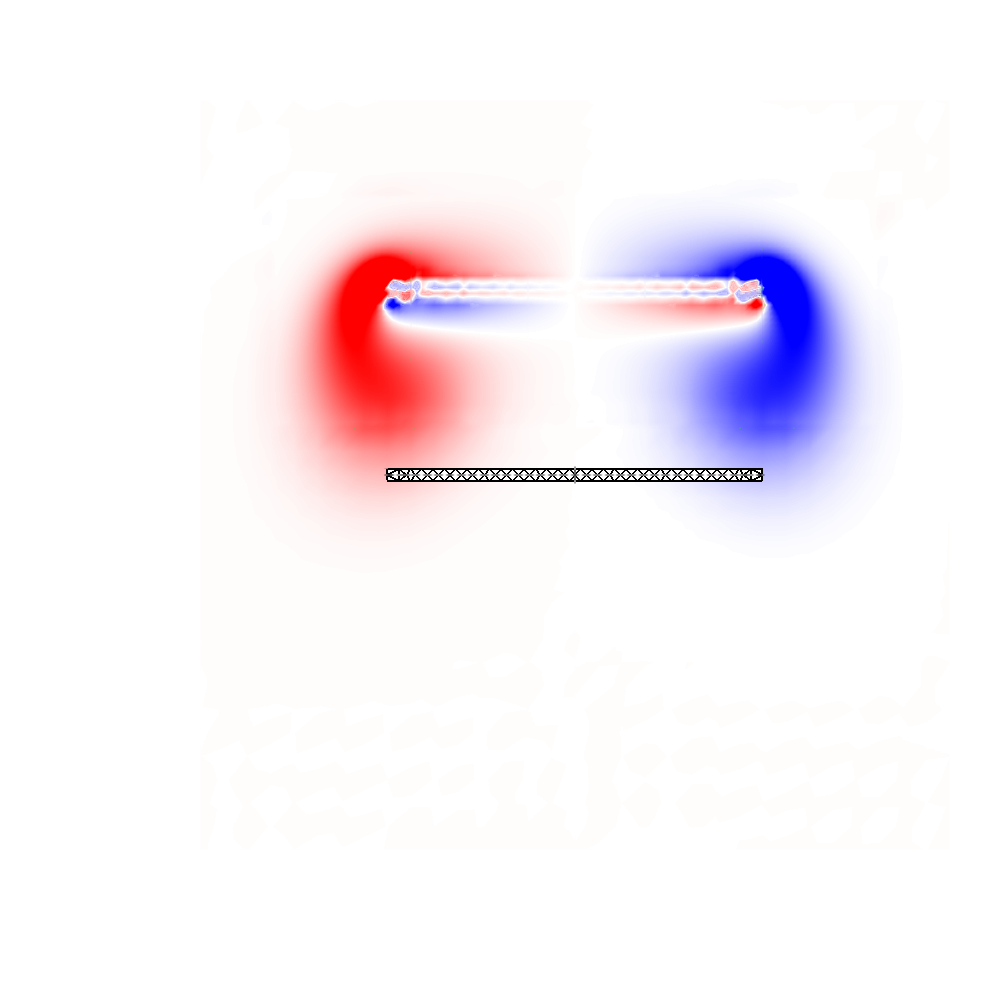
\includegraphics[width=0.33\textwidth]{ch17-full-t1-nodisplace.png}\hfill
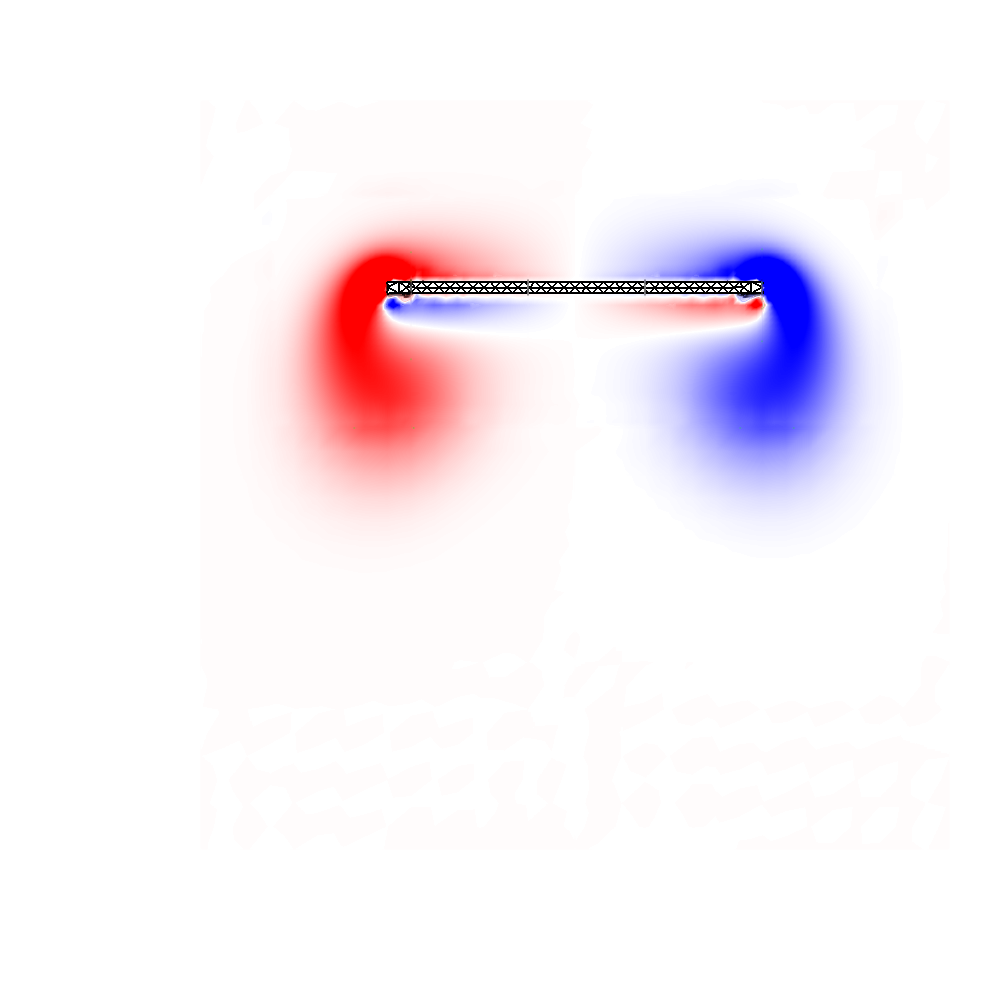
\includegraphics[width=0.33\textwidth]{ch17-full-t1.png}\\
\scriptsize IBFE/01 FULL at $t = 1$: before and after the Displace operator (chapter 17's pictures).
\end{center}
\scriptsize
\begin{itemize}
  \item Hoover's 2013 steps, in 3.5's words. The old ``Project'' step (\gui{Operators $\to$ Transforms $\to$ Project}, xy-plane by default; ``you can change this if you want if you double click Project in the collapsed menu from the Mesh Object'') was for output that stored 2D meshes with three coordinates; it is not needed now and does nothing harmful if applied.
  \item Save the session (\gui{File $\to$ Save session}) once the plots are right; restoring it with sources on the next run replaces steps 2--5.
\end{itemize}
\end{columns}
\end{frame}

% 15
\begin{frame}{The windows (2013)}
\label{fr:windows}
\begin{columns}[T]
\column{0.3\textwidth}\centering
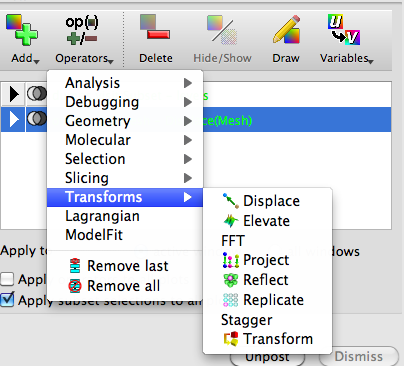
\includegraphics[width=0.8\textwidth]{ch28-h13-transforms.png}\\
\scriptsize \gui{Operators $\to$ Transforms $\to$ Displace}
\column{0.36\textwidth}\centering
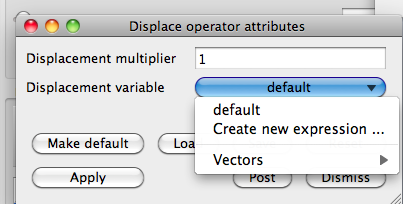
\includegraphics[width=0.85\textwidth]{ch28-h13-displace-attr.png}\\
\scriptsize the Displace attributes: multiplier, variable (\gui{default}, \gui{Create new expression}, \gui{Vectors $\to$})
\column{0.3\textwidth}\centering
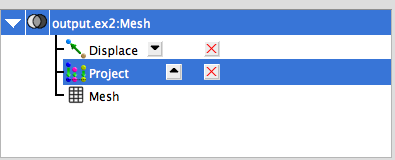
\includegraphics[width=0.8\textwidth]{ch28-h13-plotlist.png}\\
\scriptsize the plot list with Displace and the old Project on the Mesh plot
\end{columns}
\vspace{1mm}
\begin{columns}[T]
\column{0.42\textwidth}\centering
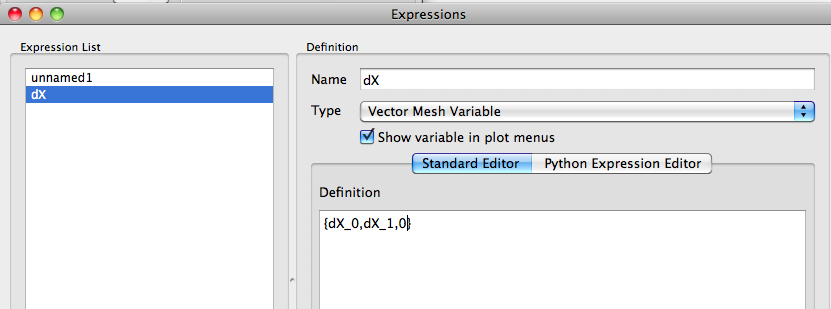
\includegraphics[width=0.7\textwidth]{ch28-h13-expression.png}\\
\scriptsize the Expressions window: \code{dX}, Vector Mesh Variable, \code{\{dX\_0, dX\_1, 0\}} (the 2013 3-component form)
\column{0.42\textwidth}\centering
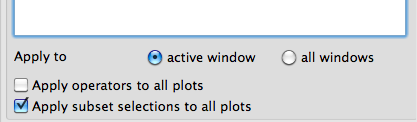
\includegraphics[width=0.7\textwidth]{ch28-h13-apply.png}\\
\scriptsize the two checkboxes under the plot list: untick the first
\end{columns}
\sourcecredit{A. Hoover, IBAMR Finite Element Visualization with VisIt (2013), VisIt 2.x on a Mac; the same windows in 3.5 with the Vector submenu filled in.}
\end{frame}

% 15b
\begin{frame}{The windows (2013), continued: the folder}
\label{fr:windows2}
\begin{columns}[T]
\column{0.5\textwidth}\centering
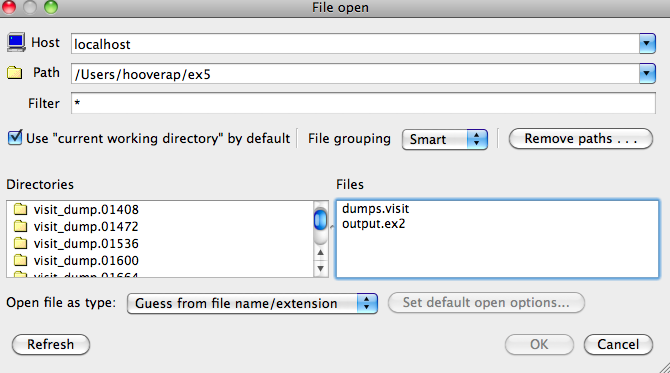
\includegraphics[width=0.95\textwidth]{ch28-h13-open.png}\\
\scriptsize the File open window of 2013: \code{dumps.visit} and \code{output.ex2} beside the \code{visit\_dump.NNNNN} folders
\column{0.48\textwidth}
\footnotesize
\begin{itemize}
  \item The window documents the folder layout of an IBFE run as it was in 2013 and still is: the fluid frames as \code{visit\_dump.NNNNN} folders listed by \code{dumps.visit}, and the one Exodus file beside them; the path (\code{/Users/hooverap/ex5}) records that the walk-through was made on upstream ex5, the cylinder.
  \item Open the two files one after the other (\gui{Open} twice); the second open asks for the database correlation (chapter 26); each becomes an entry of the \gui{Active source} list.
  \item ``Open file as type: Guess from file name/extension'' is right for both; the \code{.ex2} extension selects the Exodus reader, \code{.visit} the SAMRAI one.
\end{itemize}
\end{columns}
\sourcecredit{A. Hoover (2013), VisIt 2.x on a Mac.}
\end{frame}

% 16
\begin{frame}[fragile]{``Apply operators to all plots'': the error you get}
\label{fr:applyall}
\footnotesize
\begin{columns}[T]
\column{0.5\textwidth}
\begin{lstlisting}[style=tiny]
VisIt: Error - Pseudocolor:  ()
viewer: An invalid variable (dX) was specified.
\end{lstlisting}
\scriptsize What VisIt 3.5 says when the Displace operator with variable \code{dX} lands on the fluid's Pseudocolor plot as well: \code{dX} exists on the Exodus mesh, not on \code{amr\_mesh}, so the fluid plot cannot be drawn and nothing appears. (Reproduced on purpose; \code{wsl/final/visit\_ch28.sh}.)
\column{0.48\textwidth}
\scriptsize
\begin{itemize}
  \item The checkbox is a convenience for windows whose plots share a database. With two sources it is a trap, which is why every version of the recipe starts with ``untick''.
  \item Fix: select the fluid plot, \gui{Operators $\to$ Remove last} (or \gui{Remove all}), untick the box, re-apply Displace to the mesh plots.
  \item The reverse mistake, Displace on the Mesh but a Pseudocolor of \code{F\_1} on the same file without it: the colours are drawn on the reference mesh while the Mesh plot has moved. Every plot that should move gets its own Displace (slide \ref{fr:colour}).
  \item The multiplier is a scale on \code{dX}: 1 shows the true position; 10 exaggerates a small deformation (useful on stiff bodies, but say so on the figure); 0 is the reference mesh again.
\end{itemize}
\end{columns}
\end{frame}

% 17
\begin{frame}{Colouring the mesh by its own fields}
\label{fr:colour}
\begin{columns}[T]
\column{0.5\textwidth}\centering
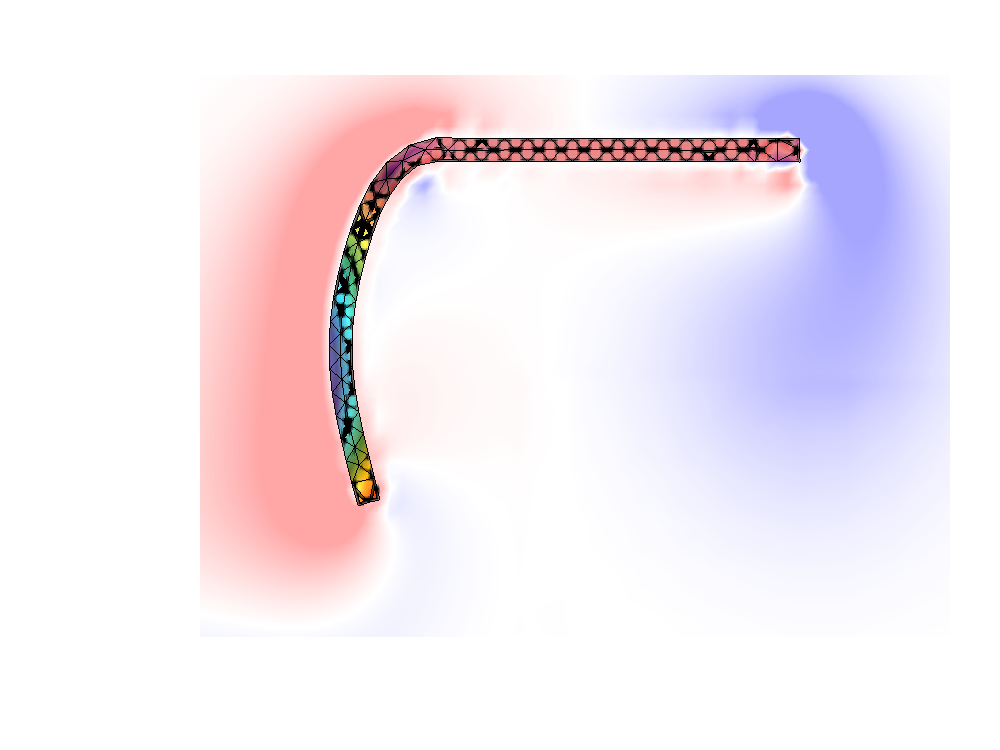
\includegraphics[width=0.74\textwidth]{ch28-ex-dxmag-t1.png}\\
\scriptsize IBFE/01 HALF at $t = 1$: \code{magnitude(dX)} ($0.25$ to $0.5$) on the displaced plate over the vorticity; the tethered right half has moved $0.5$ up, the free left half hangs from it (the README's $39^\circ$ tip-to-tip tilt). The query on this Pseudocolor plot: $|\mathbf{dX}|$ from $0.271$ (the hanging half's middle) to $0.501$, mean $0.434$.
\column{0.5\textwidth}\centering
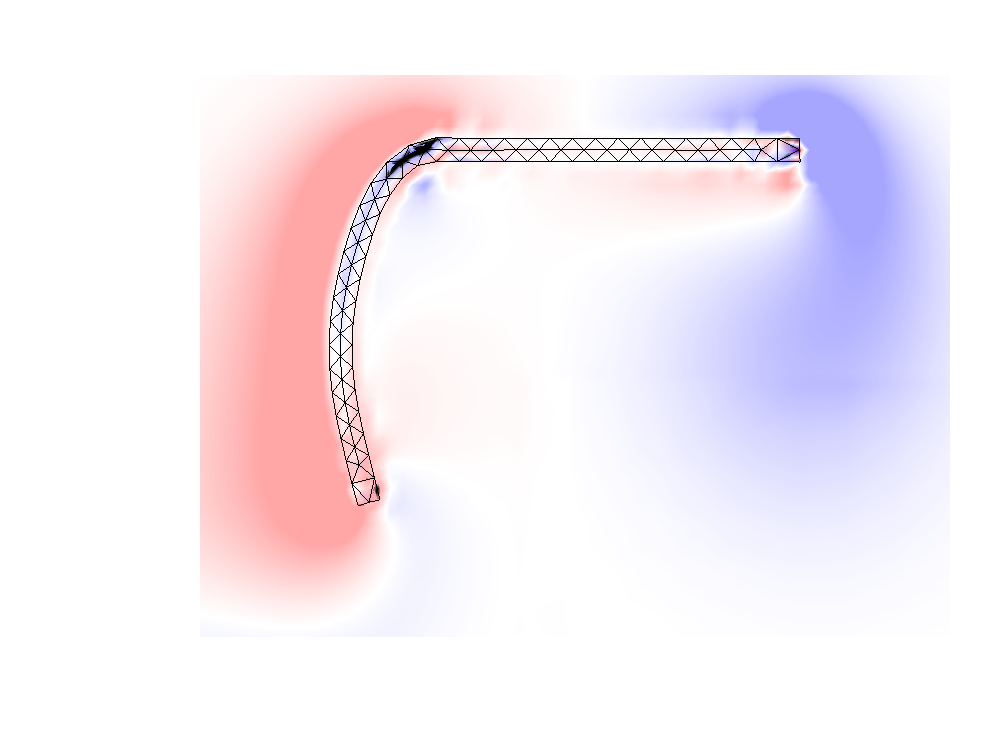
\includegraphics[width=0.74\textwidth]{ch28-ex-f1-t1.png}\\
\scriptsize the same frame, \code{F\_1} (the vertical force density, $\pm 800$) on the plate: from $-758$ at the tethered tip (node 0, pulled back against the tether's overshoot) to $+1122$ at the next node, and near zero on the free half, which carries no tether.
\end{columns}
\end{frame}

% 17b
\begin{frame}{Colouring the mesh: how}
\label{fr:colour2}
\footnotesize
\begin{itemize}
  \item With the Exodus file as the active source, \gui{Add $\to$ Pseudocolor $\to$ dX\_mag} (an expression, \code{magnitude(dX)}; or any of \code{dX\_0}, \code{U\_1}, \code{F\_0}, \ldots\ directly), then \gui{Operators $\to$ Transforms $\to$ Displace} on \emph{this} plot too; the Mesh plot on top with \gui{Opaque mode: Off} draws the edges over the colours. Fix the limits (\gui{Minimum}, \gui{Maximum}) as in chapter 26, or the colours flicker from frame to frame.
  \item \code{F} is the force density the structure exerts on the fluid at the node (per unit reference area in 2D); its sign and size tell where the tether works hardest. \code{U} is the velocity the node actually has, interpolated from the fluid.
  \item Nodal variables on a triangle mesh are interpolated linearly across each element: there is no centering choice to make, unlike chapter 26's fluid fields; a thin plate needs a zoom (this window is $1 \times 0.75$ of a $2 \times 2$ box) or thicker lines before the colours can be seen at all.
  \item The fluid's vorticity behind it is a Pseudocolor on \code{dumps.visit} with its opacity lowered (\gui{Opacity} $35\%$), so the structure's colours stay readable.
\end{itemize}
\end{frame}


% 18
\begin{frame}{Vectors on the mesh}
\label{fr:vectors}
\begin{columns}[T]
\column{0.46\textwidth}\centering
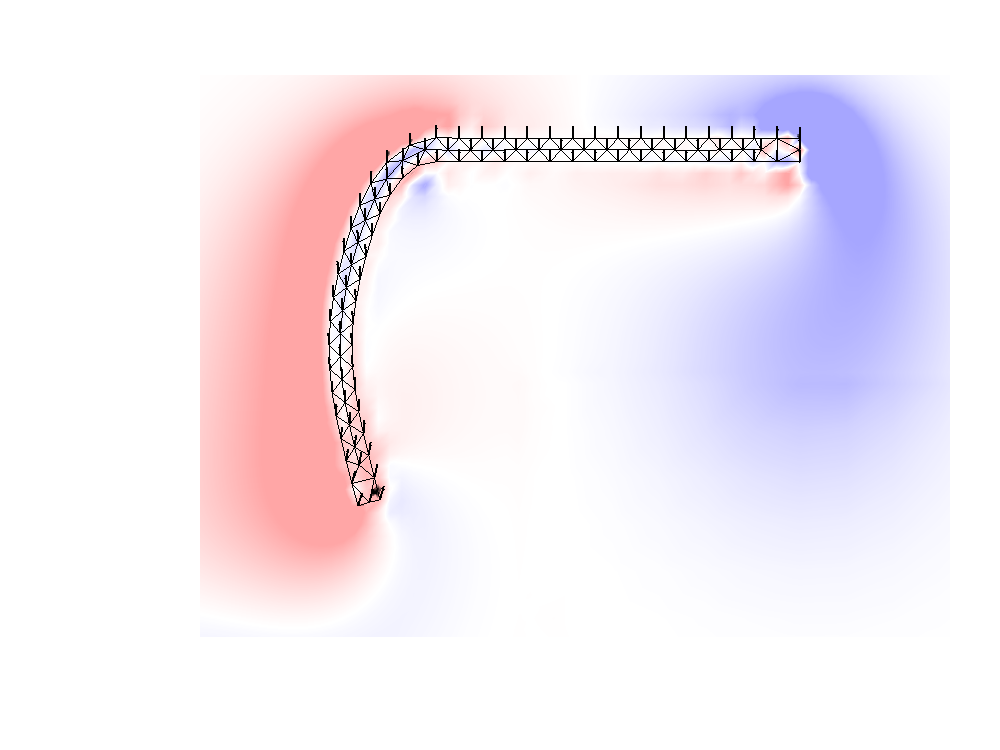
\includegraphics[width=0.9\textwidth]{ch28-ex-uvec-t1.png}
\column{0.52\textwidth}
\footnotesize
\begin{itemize}
  \item \gui{Add $\to$ Vector $\to$ U} on \code{output.ex2}, every node (\gui{Stride} 1), one colour, with the Displace operator on the Vector plot too: the plate's velocity at $t = 1$ (HALF: the tethered half moves at the prescribed $0.5$, the free half swings at up to $0.61$; the \gui{MinMax} query on the Vector plot gives $0.4997$ to $0.608$).
  \item The Vector plot draws one glyph per node of the mesh (101 here), so \gui{Stride} 1 is right on a structure, where chapter 26 thinned the fluid's vectors to a few thousand; \gui{Scale} sets the arrow length in data units (0.12 here).
  \item The Vector plot of \code{F} shows the force density the same way; on a tethered plate it is large only where the tether pulls.
  \item In 3D the expression must be built first (\code{\{U\_0, U\_1, U\_2\}}, slide \ref{fr:threed}).
\end{itemize}
\end{columns}
\end{frame}

% 18b
\begin{frame}{The mesh's own quality}
\label{fr:quality}
\begin{center}
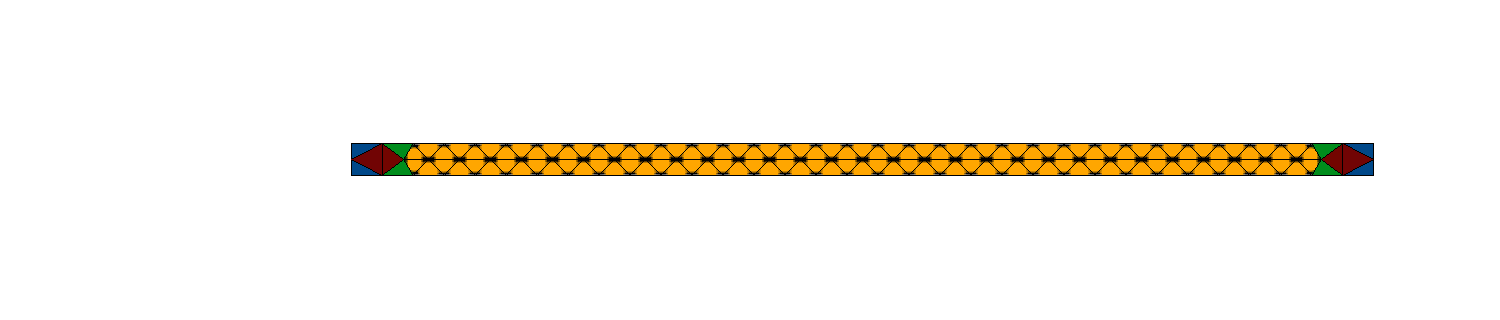
\includegraphics[width=0.8\textwidth]{ch28-ex-aspect.png}\\
\scriptsize \code{mesh\_quality/minimum\_angle} of the plate's 130 triangles at the reference state, $27^\circ$ to $54^\circ$ (the \code{aspect} measure returns $0$ on triangles in 3.5; \code{condition} runs from $1.007$ to $1.42$): the expressions VisIt attaches to every mesh.
\end{center}
\footnotesize
\begin{itemize}
  \item \code{mesh\_quality/*} are computed from the geometry at the current state: at the reference state they judge the mesher's work (chapter 18 for the element size, chapter 22's sliver slide for the shape: angles well away from $0$ and $180^\circ$, no slivers); at a later state, \code{jacobian} or \code{scaled\_jacobian} going to zero shows an element that has been crushed, and \code{area} (\code{volume} in 3D) against its reference value is the local $J$ of chapter 19.
  \item A Threshold on one of them (slide \ref{fr:select}) isolates the bad elements; the 3D plate of chapter 22 with its sliver tetrahedra is on slide \ref{fr:threed}.
\end{itemize}
\end{frame}

% 18c
\begin{frame}{The \code{mesh\_quality} expressions, 2D and 3D}
\label{fr:quality2}
\footnotesize
\begin{itemize}
  \item The 2D list (from the file's metadata): \code{area}, \code{aspect}, \code{condition}, \code{degree}, \code{jacobian}, \code{max\_edge\_length}, \code{maximum\_angle}, \code{min\_edge\_length}, \code{min\_corner\_area}, \code{min\_sin\_corner}, \code{min\_sin\_corner\_cw}, \code{minimum\_angle}, \code{neighbor}, \code{oddy}, \code{relative\_size}, \code{scaled\_jacobian}, \code{shape}, \code{shape\_and\_size}, \code{shear}, \code{skew}, \code{stretch}, \code{taper}, \code{warpage}. The 3D list drops \code{area}, the angle measures, \code{min\_corner\_area}, \code{min\_sin\_corner(\_cw)} and \code{warpage}, and adds \code{aspect\_gamma}, \code{diagonal\_ratio}, \code{min\_diagonal}, \code{max\_diagonal}, \code{dimension}, \code{max\_side\_volume}, \code{min\_side\_volume}, \code{node\_degree}, \code{volume}, \code{face\_planarity}, \code{relative\_face\_planarity}: in 3D judge tetrahedra by \code{aspect\_gamma}, \code{condition} or \code{shape}.
  \item Each is a zonal scalar (one value per element), so a Pseudocolor of it colours elements, and a Threshold on it keeps elements; the Query window's \gui{Min}/\gui{Max} give the worst element and its position.
  \item They are VisIt's (the Verdict library), not IBAMR's: the same names appear on any mesh VisIt opens, including the fluid's \code{amr\_mesh}, where they say nothing useful (every cell is a square).
\end{itemize}
\end{frame}


% 19
\begin{frame}[fragile]{Pick: numbers at one node}
\label{fr:pick}
\footnotesize
\begin{columns}[T]
\column{0.46\textwidth}
\begin{lstlisting}[style=tiny]
B:  output.ex2  timestep 10        # IBFE/01 FULL, t = 1
Mesh
Point: <0.5, 0>                    # reference position
Node:  0
Incident Zones:  0  1  3
X_0:  <nodal> = 0.499631
X_1:  <nodal> = 0.500316
dX_0:  <nodal> = -0.000369177
dX_1:  <nodal> = 0.500316
U_0:  <nodal> = 0.00198706
U_1:  <nodal> = 0.510143
F_0:  <nodal> = 530.064
F_1:  <nodal> = -652.487
\end{lstlisting}
\column{0.52\textwidth}
\scriptsize
\begin{itemize}
  \item \gui{Controls $\to$ Pick}, \gui{Node} or \gui{Zone} mode, choose the variables to report, click on the plot (or type a node number in the window's \gui{Pick by node} field). The output above is the CLI's \code{PickByNode(0, 0, (...))}: node 0 is the plate's right tip, at the reference point $(0.5, 0)$; at $t = 1$ it sits at $(0.4996, 0.5003)$, moving up at $0.51$, pushed by a tether force of $(530, -652)$.
  \item The reported \gui{Point} is always the \emph{reference} (file) position, with or without the Displace operator on the plot; the mouse pick is made in the displayed geometry, so click where you look, and read the current position from \code{X\_0}, \code{X\_1}.
  \item \gui{Do time curve}: the next pick produces the chosen variables of that node against time in window 2, a Curve plot that \gui{File $\to$ Save window} exports as text (slide \ref{fr:curve}). This is how the IBFE/01 README's tip positions were read.
  \item Node numbers are libMesh's (0-based here; \code{node\_num\_map} holds the file's own ids). To find a node by position, pick it once with the mouse; the number is then yours for scripts.
\end{itemize}
\end{columns}
\end{frame}

% 20
\begin{frame}{Query over time: a field's maximum, minimum or mean against time}
\label{fr:qot}
\begin{columns}[T]
\column{0.5\textwidth}\centering
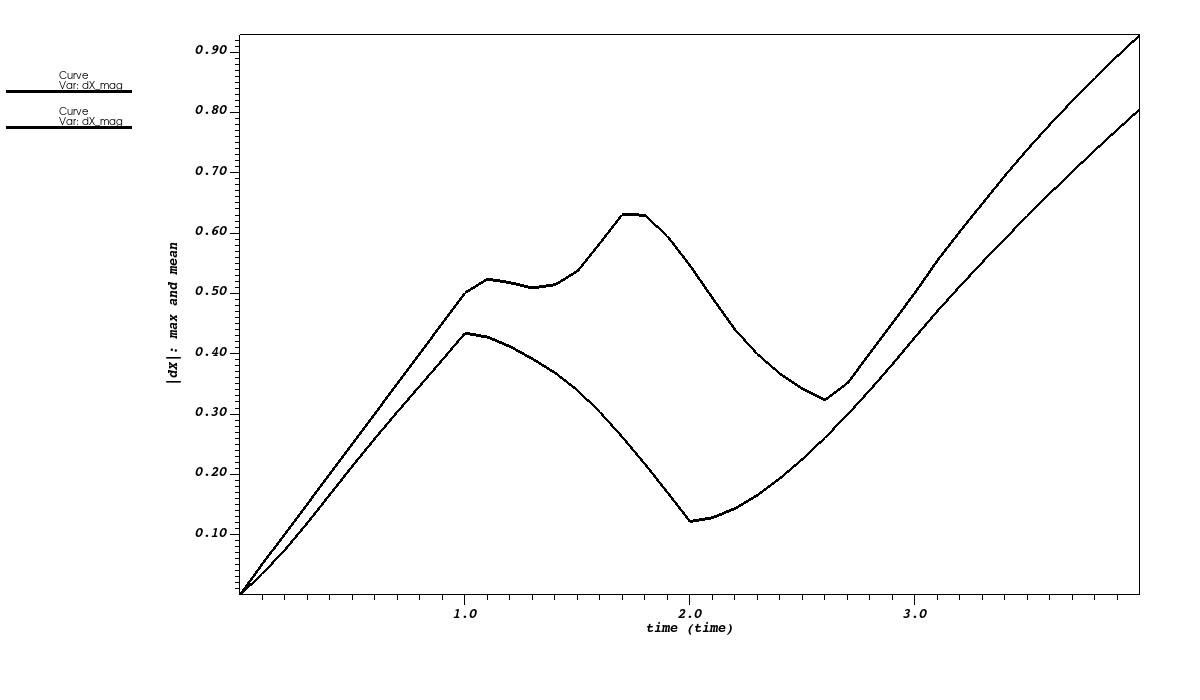
\includegraphics[width=0.84\textwidth]{ch28-ex-qot.png}\\
\scriptsize Window 2 after two time queries on \code{magnitude(dX)} of IBFE/01 HALF: the maximum (the tethered tip's prescribed path) and the average over the plate. The maximum follows the prescribed tether only up to $t = 1$ ($0.05$ per $0.1$ s to $0.50$); from $t \approx 1.1$ the swinging free half moves further than the tethered tip, so the maximum stays above $0.3$ ($0.55$ at $t = 2$, $0.32$ at $t = 2.6$, $0.50$ at $t = 3$ when the tether reaches $-0.5$) and climbs to $0.93$ at $t = 4$ after the release at $t = 3$; the mean lags it. The \code{.curve} file on slide \ref{fr:curve} is this window.
\column{0.48\textwidth}
\footnotesize
\begin{enumerate}
  \item \gui{Controls $\to$ Query over time options}: x-axis \gui{Time} (called \gui{DTime} in the Python attributes; \gui{Cycle} and \gui{Timestep} are the alternatives), start, end and stride if not the whole run.
  \item Select the Pseudocolor plot of the variable (a Mesh plot cannot be queried: ``Cannot perform a Max query on variable Mesh''); it must be visible (``cannot be hidden'', 2014) and needs no Displace operator (``no need to displace at the moment'': queries read the fields, pictures need the operator).
\end{enumerate}
\end{columns}
\end{frame}

% 20b
\begin{frame}{Query over time (2): the query, and the window it lands in}
\label{fr:qot2}
\footnotesize
\begin{enumerate}
  \setcounter{enumi}{2}
  \item \gui{Controls $\to$ Query}: \gui{Display: All queries-over-time}, pick \gui{Max}, \gui{Min} or \gui{Average Value}, tick \gui{Do Time Query}, \gui{Query}.
  \item The result opens window 2 as a Curve plot (``this may take a while'' over many states; ``terrible UI decision'' in the 2014 deck: subsequent queries go into the same window, ``can probably be fixed using Python''; in 3.5 the Query over time options have the window settings for it). The curve window is bare by default: \gui{Controls $\to$ Annotation} (the deck's ``Control>Annotations'') sets its title, axes and legend before \gui{File $\to$ Save window}.
\end{enumerate}
\end{frame}

% 21
\begin{frame}{The 2014 windows: queries}
\label{fr:windows14}
\begin{columns}[T]
\column{0.26\textwidth}\centering
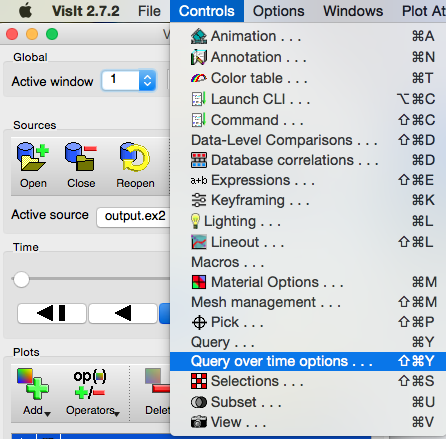
\includegraphics[width=0.9\textwidth]{ch28-h14-controls.png}\\
\scriptsize \gui{Controls $\to$ Query over time options}
\column{0.26\textwidth}\centering
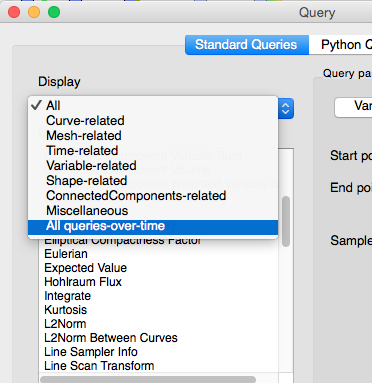
\includegraphics[width=0.9\textwidth]{ch28-h14-query-display.png}\\
\scriptsize the Query window, \gui{Display: All queries-over-time}
\column{0.22\textwidth}\centering
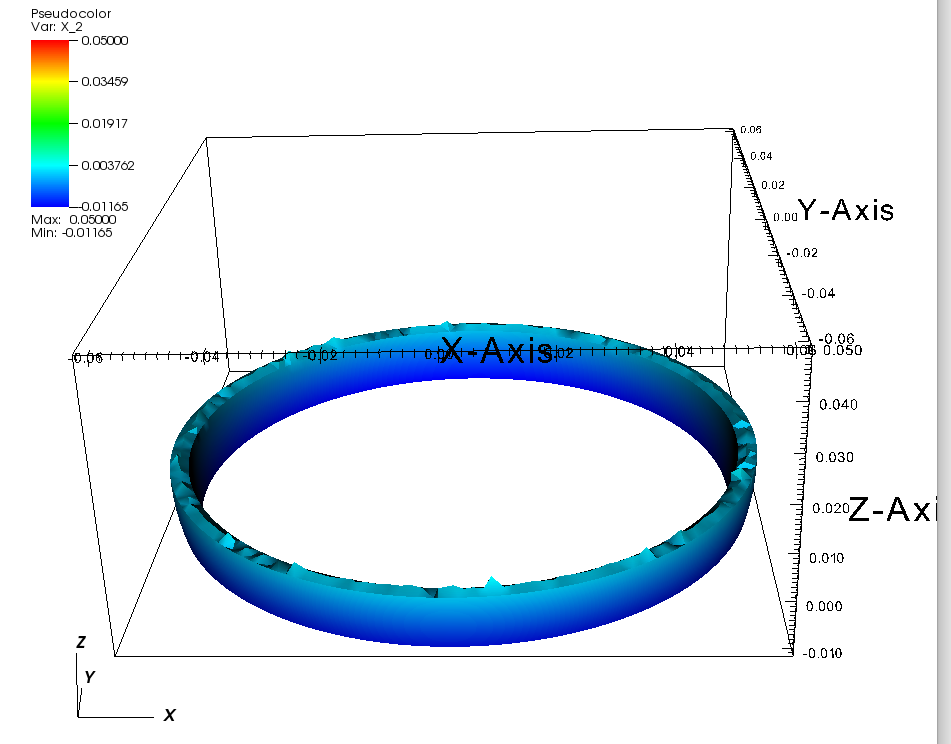
\includegraphics[width=0.9\textwidth]{ch28-h14-bell.png}\\
\scriptsize the bell ring coloured by \code{X\_2}, its $z$ position (slide 7)
\column{0.24\textwidth}\centering
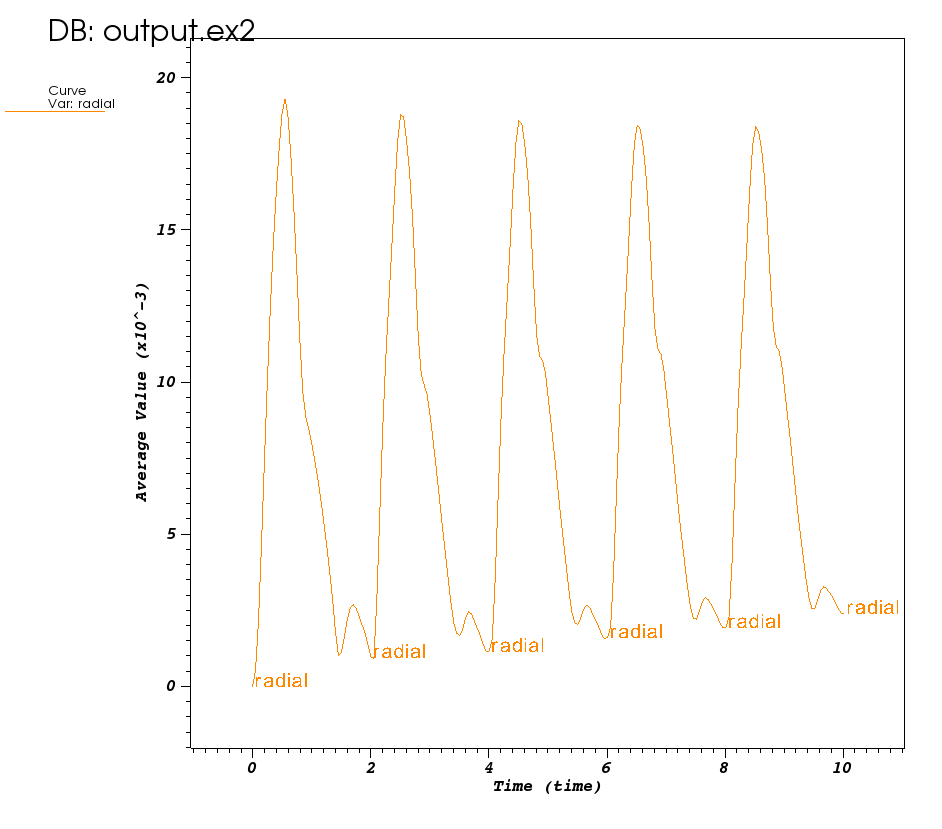
\includegraphics[width=0.9\textwidth]{ch28-h14-curve-radial.png}\\
\scriptsize the curve window
\end{columns}
\scriptsize The 2014 deck did this on a jellyfish bell (a 3D ring mesh): the average $z$ position \code{X\_2} of the bell (slide 6) and the average of its ``radial'' expression over $z < 0.01$ (slide 9), with the windows above.
\sourcecredit{A. Hoover, 5-IBFE Tutorial: Visualizing Lagrangian Data (2014), VisIt 2.7.2 on a Mac.}
\end{frame}

% 21b
\begin{frame}{The 2014 windows: plots and expressions}
\label{fr:windows14b}
\begin{columns}[T]
\column{0.25\textwidth}\centering
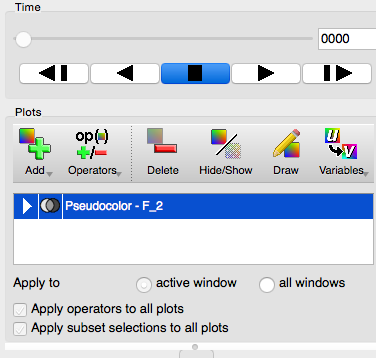
\includegraphics[width=0.9\textwidth]{ch28-h14-main.png}\\
\scriptsize the main window with \code{F\_2}
\column{0.25\textwidth}\centering
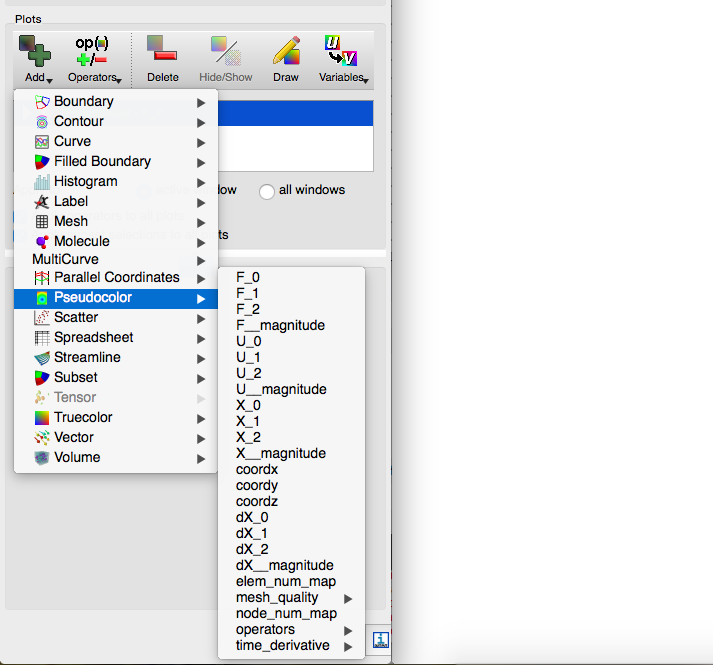
\includegraphics[width=0.9\textwidth]{ch28-h14-pc-menu.png}\\
\scriptsize \gui{Add $\to$ Pseudocolor} on an Exodus file
\column{0.25\textwidth}\centering
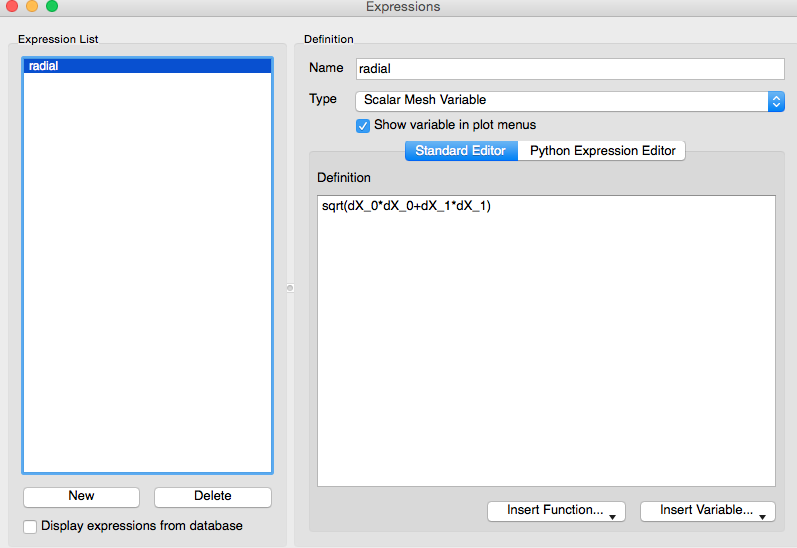
\includegraphics[width=0.9\textwidth]{ch28-h14-expression.png}\\
\scriptsize the Expressions window (``radial'')
\column{0.25\textwidth}\centering
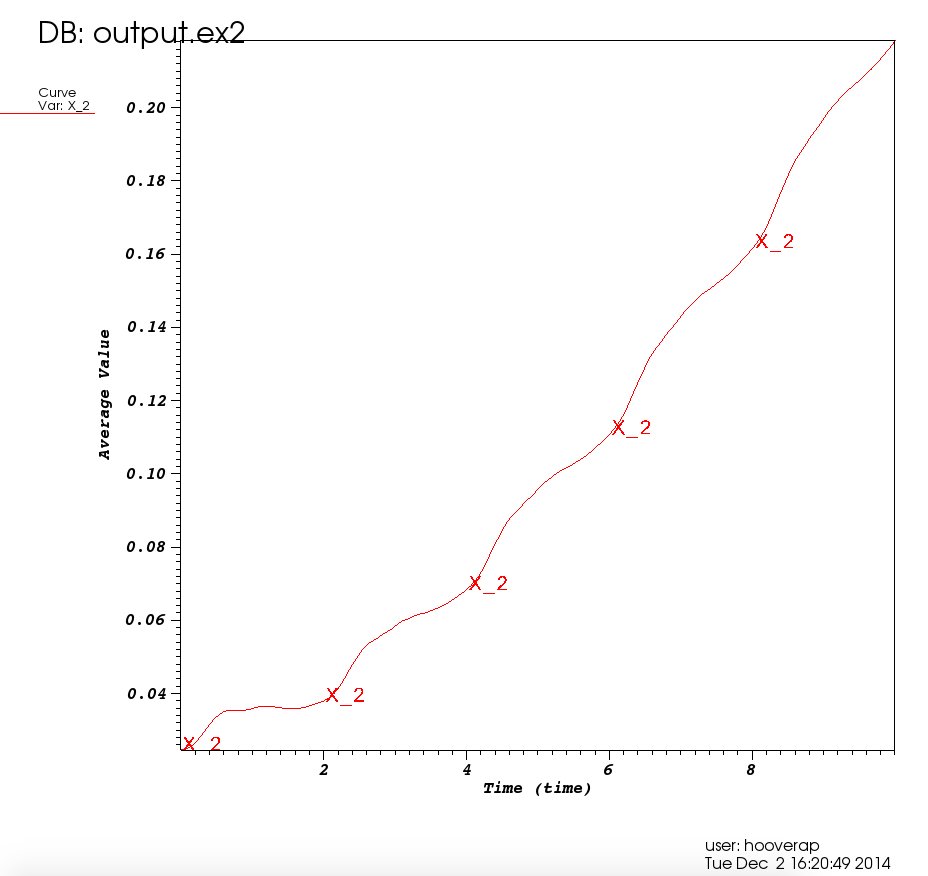
\includegraphics[width=0.9\textwidth]{ch28-h14-curve-uz.png}\\
\scriptsize slide 6: the average \code{X\_2} of the bell against time in window 2
\end{columns}
\sourcecredit{A. Hoover (2014), VisIt 2.7.2. The Pseudocolor menu already lists \code{F\_magnitude} and \code{U\_magnitude}: VisIt's reader built the vectors then too.}
\end{frame}


% 22
\begin{frame}{Selections: querying part of the structure}
\label{fr:select}
\begin{columns}[T]
\column{0.33\textwidth}\centering
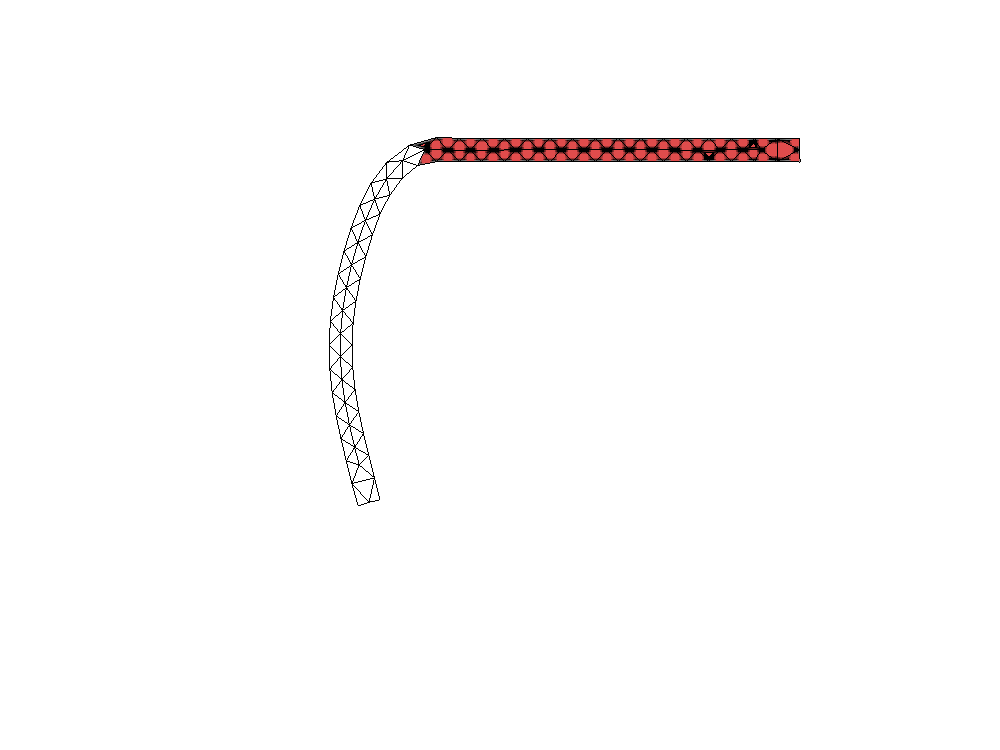
\includegraphics[width=0.9\textwidth]{ch28-ex-box-t1.png}\\
\scriptsize \gui{Operators $\to$ Selection $\to$ Box}, $x \in [0, 1]$: the right half
\column{0.33\textwidth}\centering
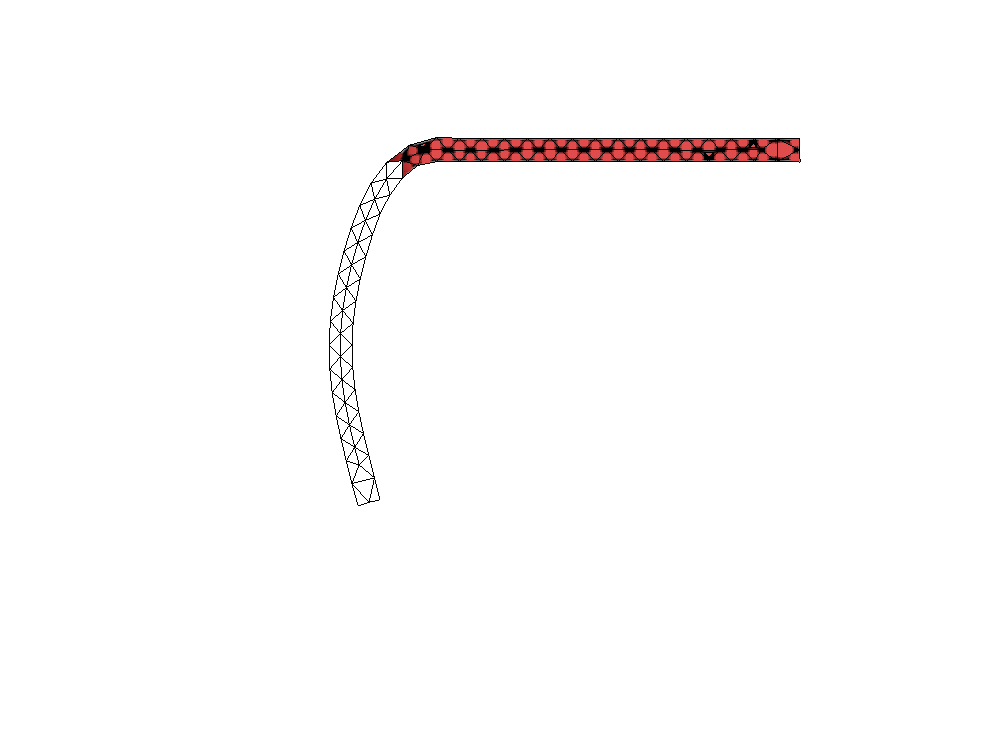
\includegraphics[width=0.9\textwidth]{ch28-ex-threshold-t1.png}\\
\scriptsize \gui{Threshold} on \code{dX\_mag} $\ge 0.49$: the nodes that moved the full way
\column{0.33\textwidth}\centering
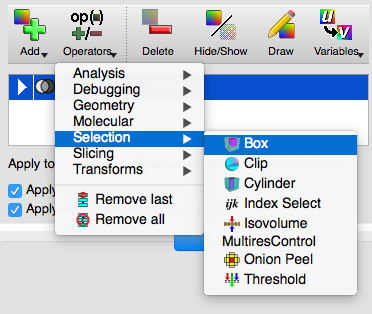
\includegraphics[width=0.9\textwidth]{ch28-h14-selection-menu.png}\\
\scriptsize the Selection submenu (2014)
\end{columns}
\footnotesize
\begin{itemize}
  \item A selection operator keeps part of the data; every query after it acts on what is left. On the HALF plate at $t = 1$: the Box $x \in [0, 1]$, applied after Displace so it acts on the current positions, keeps $53$ of the $101$ nodes ($66$ of $130$ triangles) with mean $|\mathbf{dX}| = 0.4999$; the Threshold $|\mathbf{dX}| \ge 0.49$ keeps $56$ nodes and $70$ triangles, mean $0.4993$: the tethered half and the fold.
\end{itemize}
\end{frame}

% 22b
\begin{frame}{The selection operators}
\label{fr:select2}
\footnotesize
\begin{itemize}
  \item \gui{Box} takes ranges in $x$, $y$ and $z$ (``you must specify range in x, y and z'', the 2018 deck, of a 3D run; the window asks for $z$ in 2D too, and a range containing $0$ is harmless); \gui{Clip} a half-space or a sphere; \gui{Threshold} a range of a variable (zonal: keep an element when all, or part, of its nodes qualify: \gui{Show zone if: Part in range / All in range}, \code{zonePortions} in Python); \gui{Isovolume} the same for a continuous field; \gui{Index Select} and \gui{Onion Peel} by numbering and adjacency; \gui{Cylinder} a tube (3D).
  \item The 2014 deck selected the bell's lower half ``for $z \le 0$'' on one slide and ``$z < 0.01$'' on another, naming the operator only through its screenshot of the Selection menu with \gui{Box} highlighted; a Box (or Clip) with that $z$ range reproduces it. The ``radial component'' it then averaged is slide \ref{fr:expr}.
  \item The operator applies to the plot it is attached to, so put the selection on the Pseudocolor plot you query, and leave the Mesh plot whole if the picture should still show the entire structure.
  \item Operator order matters (top of the list is applied first): Displace then Box selects by current position; Box then Displace selects by reference position and moves what is left. The picture on the previous slide used the first order.
  \item A selection is also the way to a query on one part of a multi-part run when the parts are in one file (one block each): Threshold on \code{ElementBlock} (slide \ref{fr:blocks}).
\end{itemize}
\end{frame}


% 23
\begin{frame}[fragile]{Expressions on the mesh}
\label{fr:expr}
\footnotesize
\begin{columns}[T]
\column{0.52\textwidth}
\begin{lstlisting}[style=tiny]
# Controls > Expressions on an Exodus file (3.5 defines dX, U, F, X)
dX_mag    scalar  magnitude(dX)                   # in-plane displacement
speed     scalar  magnitude(U)
Fmag      scalar  magnitude(F)
Fn        scalar  F_1                             # one component: no expression needed
dX_rad    scalar  (dX_0*coordx + dX_1*coordy) / sqrt(coordx*coordx + coordy*coordy)
                                                  # radial about the origin, from the reference position
dX_frac   scalar  magnitude(dX) / 0.5             # relative to a prescribed amplitude
work      scalar  F_0*U_0 + F_1*U_1               # power density at the node
jac0      scalar  mesh_quality/jacobian            # element quality now
\end{lstlisting}
\column{0.46\textwidth}
\scriptsize
\begin{itemize}
  \item Hoover's 2014 ``\code{sqrt(dX\_0*dX\_0+dX\_1*dX\_1)} gives radial component'' is the in-plane displacement \emph{magnitude}; for a bell whose axis is $z$ that is the distance moved in the plane, not its radial part. The true radial component projects \code{dX} on the radial unit vector (the \code{dX\_rad} line, with \code{coordx}, \code{coordy} as the reference position; in 3D about the $z$ axis the same two components).
  \item Expression types: \emph{Scalar mesh variable} or \emph{Vector mesh variable} (the type is the menu it appears in). Vector algebra: \code{\{a, b\}}, \code{v[0]}, \code{magnitude(v)}, \code{dot(v, w)}; \gui{Insert Function} and \gui{Insert Variable} write the names for you.
  \item Expressions on the fluid and on the mesh are separate worlds: an expression that mixes \code{Omega} and \code{dX} fails (different meshes). To bring a fluid value onto the structure, VisIt's \code{pos\_cmfe} maps one mesh onto another by position; chapter 29.
\end{itemize}
\end{columns}
\end{frame}

% 24
\begin{frame}{Several parts: one file each}
\label{fr:parts}
\begin{columns}[T]
\column{0.64\textwidth}\centering
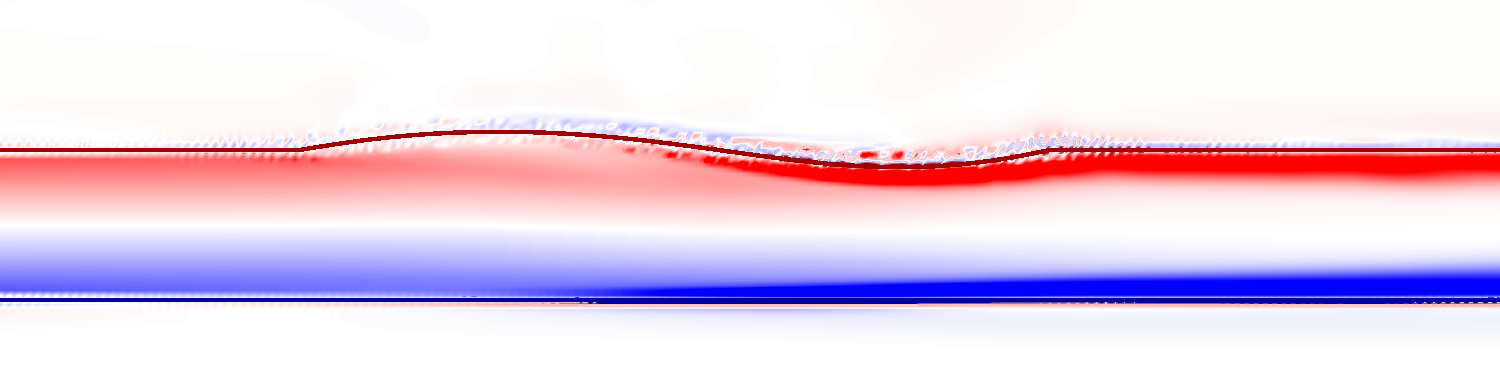
\includegraphics[width=\textwidth]{ch28-ex7-parts.png}\\
\scriptsize Upstream IBFE ex7 (chapter 23) at $t = 2$, the collapsible segment: \code{loweroutput.ex2} (blue) and \code{upperoutput.ex2} (red), each a Mesh plot with its own Displace, over the vorticity ($\pm 50$).
\column{0.34\textwidth}\centering
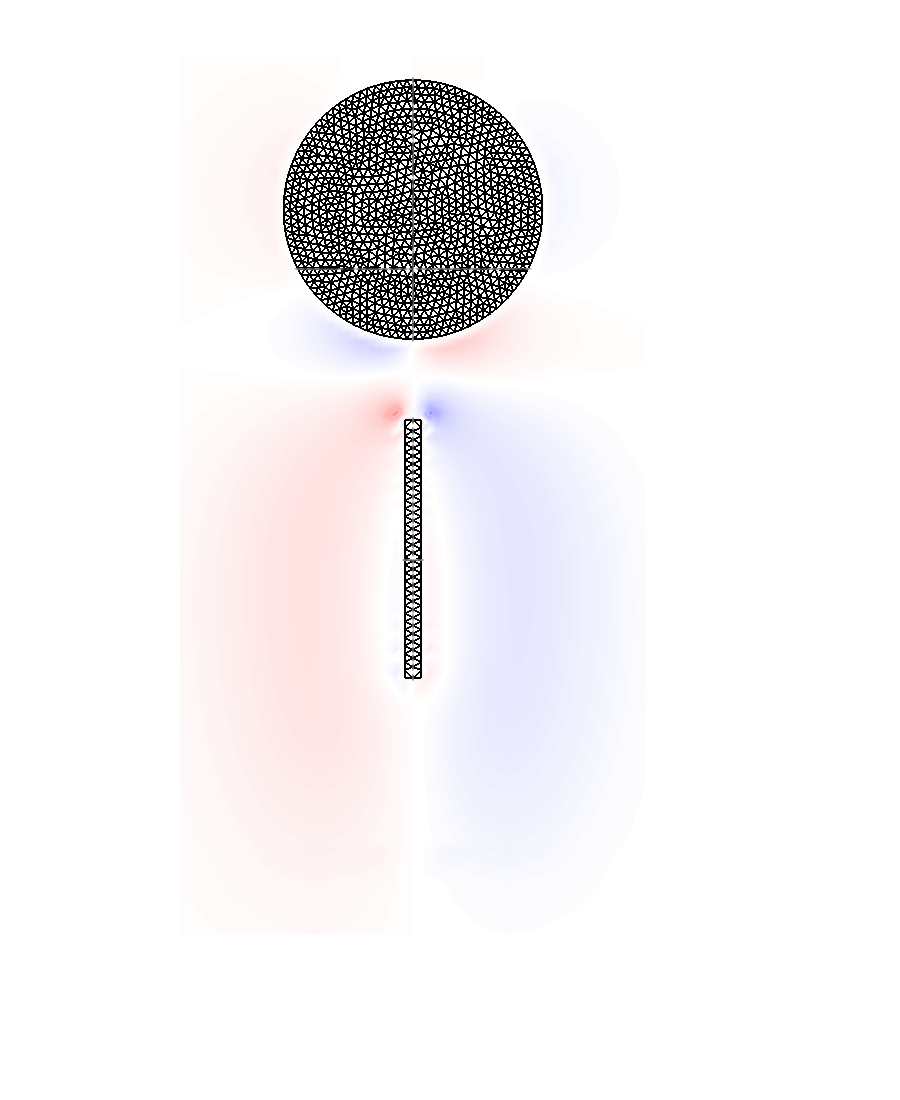
\includegraphics[width=0.5\textwidth]{ch21-hit-t2.png}\\
\scriptsize IBFE/08 (chapter 21): \code{beam\_output.ex2} and \code{circle\_output.ex2}.
\end{columns}
\footnotesize
\begin{itemize}
  \item Each part is a separate database with its own active source: \gui{Open} it, \gui{Add $\to$ Mesh}, Displace with \code{dX} (every file has the same variable names, so one expression serves all), \gui{Draw}; repeat. Colour the parts apart in the Mesh attributes (\gui{Mesh color: Custom}) or colour each by its own field.
\end{itemize}
\end{frame}

% 24b
\begin{frame}{Several parts: operators, time, queries}
\label{fr:parts2}
\footnotesize
\begin{itemize}
  \item ``Apply operators to all plots'' would put the operator on all mesh plots in one go, but also on the fluid (slide \ref{fr:applyall}); untick and apply per plot, or tick, apply, and remove it from the fluid plot (chapter 21's note).
  \item The time slider: the files written in the same run at the same interval have the same number of states and step together; \gui{Controls $\to$ Database correlations} lines up files with different cadences by time (chapter 26).
  \item Querying two parts against each other (the gap between the beam's top and the circle's bottom in IBFE/08) is not a GUI query: two picks per frame, or the two-file script of chapter 32.
  \item Upstream ex7's files also carry node sets (\code{Nodesets} in the variable list): the boundary ids that libMesh's \code{build\_square} gives the edges of each wall mesh. Its tether selects by the reference $x$ coordinate (chapter 23), not by set; a Subset of the node sets shows the mesh edges that carry an id.
  \item One part per file is IBAMR's choice, not Exodus's: a single Exodus file can hold several element blocks (slide \ref{fr:blocks}), which is what you get when one mesh file contains two bodies (chapter 21's way C).
\end{itemize}
\end{frame}


% 25
\begin{frame}{Element blocks and sets: the Subset plot}
\label{fr:blocks}
\begin{columns}[T]
\column{0.42\textwidth}\centering
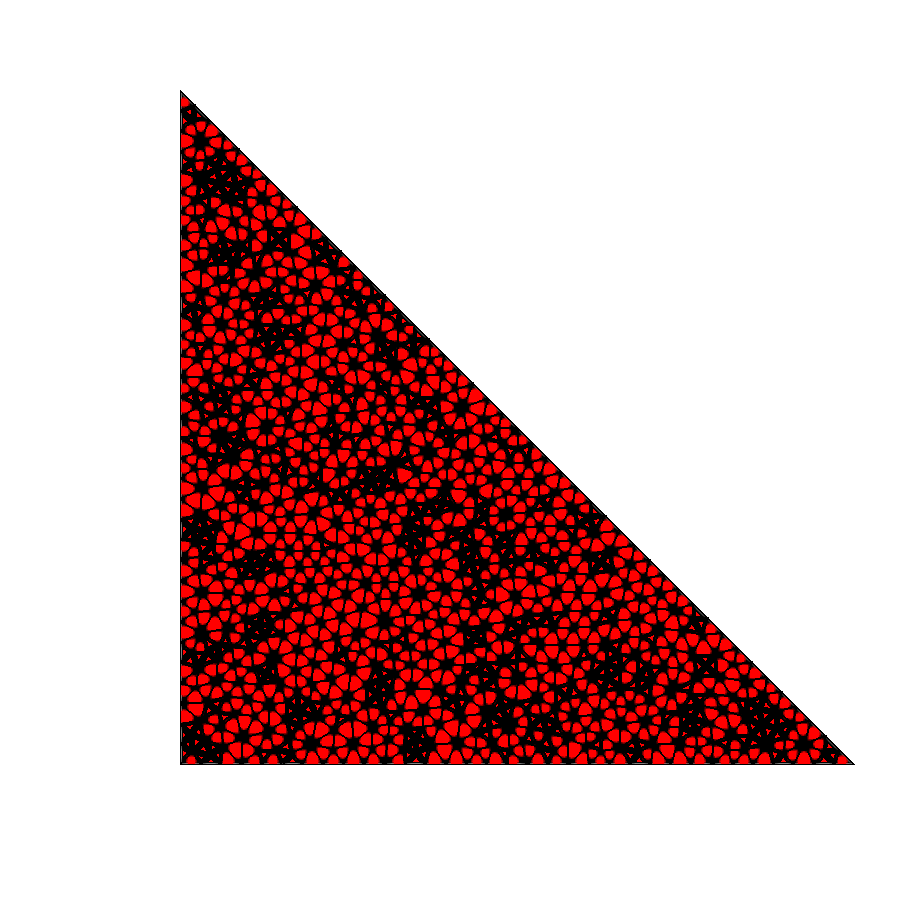
\includegraphics[width=0.9\textwidth]{ch28-ex-blocks.png}\\
\scriptsize IBFE/05's gmsh triangle (the \code{triangle\_gmsh.msh} run): the Subset plot of \code{ElementBlock} with the Mesh plot on top; one block, \code{triangle\_1}: the physical surface ``triangle'' of \code{triangle.geo}, with the block id 1 appended by VisIt.
\column{0.56\textwidth}
\footnotesize
\begin{itemize}
  \item \gui{Add $\to$ Subset $\to$ ElementBlock} colours the elements by block; the Subset window lists the blocks and can hide them. The gmsh triangle of IBFE/05 has one block named \code{triangle}: libMesh copies a gmsh physical name into the subdomain name and the Exodus block name (VisIt shows it as \code{triangle\_1}, name plus id); the course's shipped \code{triangle.msh} carries no physical name and its block is unnamed, shown by its id, like the plate's block \code{0}; the 3D plate's is \code{plate2\_1}.
\end{itemize}
\end{columns}
\end{frame}

% 25b
\begin{frame}{Element blocks and sets (2): where they come from}
\label{fr:blocks2}
\footnotesize
\begin{itemize}
  \item Blocks come from the mesh file: gmsh physical surfaces or volumes (chapter 18; libMesh maps each to a subdomain id and Exodus block), Exodus/Cubit blocks, or \code{elem->subdomain\_id()} set in the program. The IBFE/10 two-material plate of chapter 22 chose its material by position instead, so its file has one block.
  \item Node sets and side sets (gmsh physical lines, Cubit nodesets/sidesets) appear as the scalar \code{Nodesets} and as Subset categories when present: upstream ex7's walls carry them, the plate does not.
  \item A Threshold on \code{ElementBlock} (a zonal integer) is the other way to keep one block.
\end{itemize}
\end{frame}

% 26
\begin{frame}{Three dimensions: the plate of IBFE/10}
\label{fr:threed}
\begin{columns}[T]
\column{0.34\textwidth}\centering
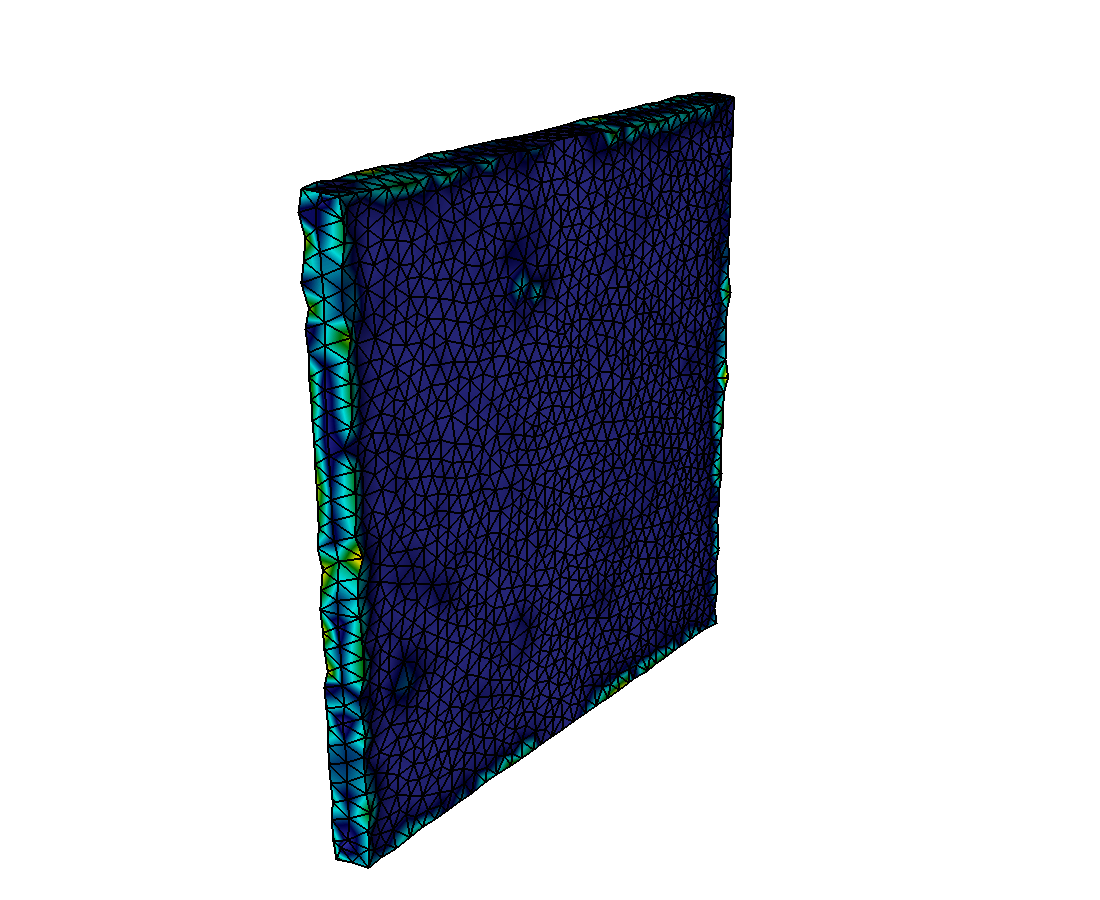
\includegraphics[width=0.82\textwidth]{ch28-3d-dx.png}\\
\scriptsize \code{magnitude(\{dX\_0, dX\_1, dX\_2\})} on the displaced plate at $t = 0.5$: maximum $0.052$ at the free edge; $3386$ nodes, $11\,481$ tetrahedra, block \code{plate2\_1}
\column{0.34\textwidth}\centering
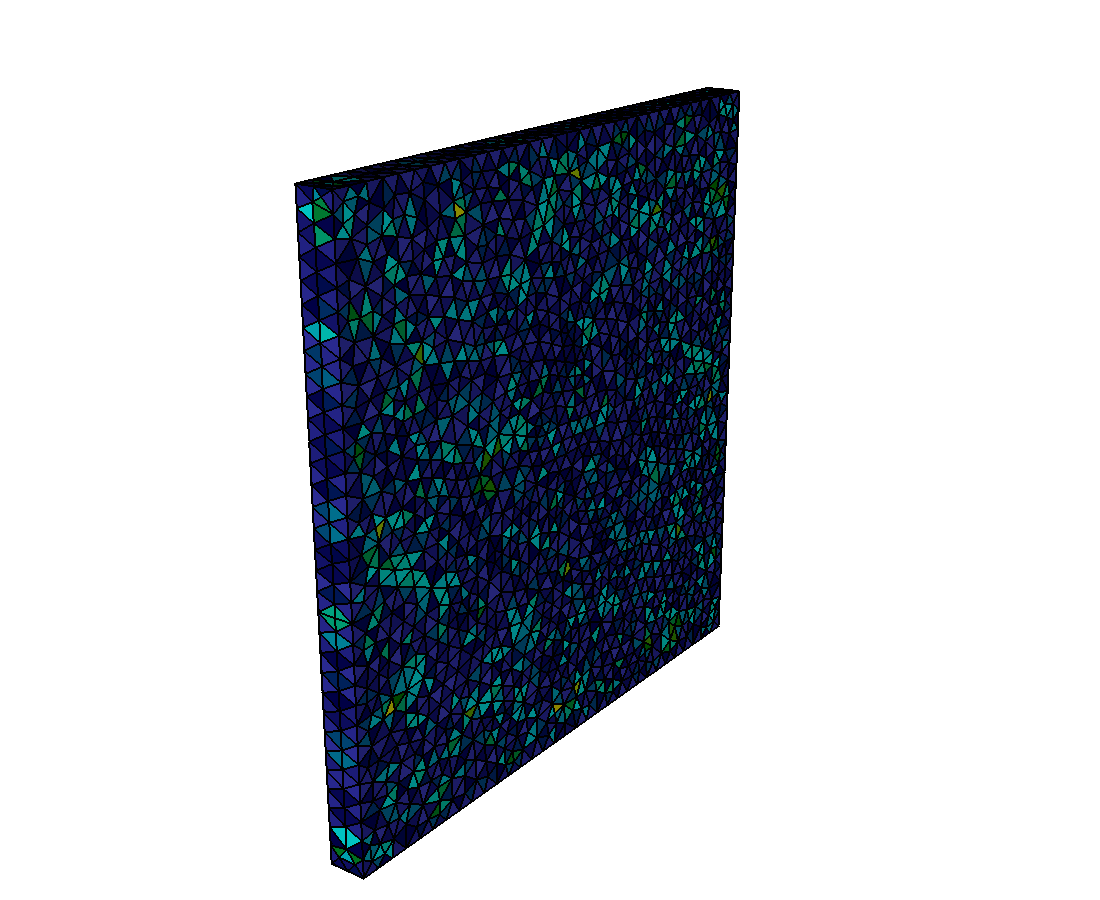
\includegraphics[width=0.82\textwidth]{ch28-3d-quality.png}\\
\scriptsize \code{mesh\_quality/aspect\_gamma} of its tetrahedra at the reference state ($1$ to $4$ shown; the range is $1.005$ to $225$: the slivers of chapter 22's note; $337$ of the $11\,481$ tetrahedra are above $4$)
\column{0.3\textwidth}\centering
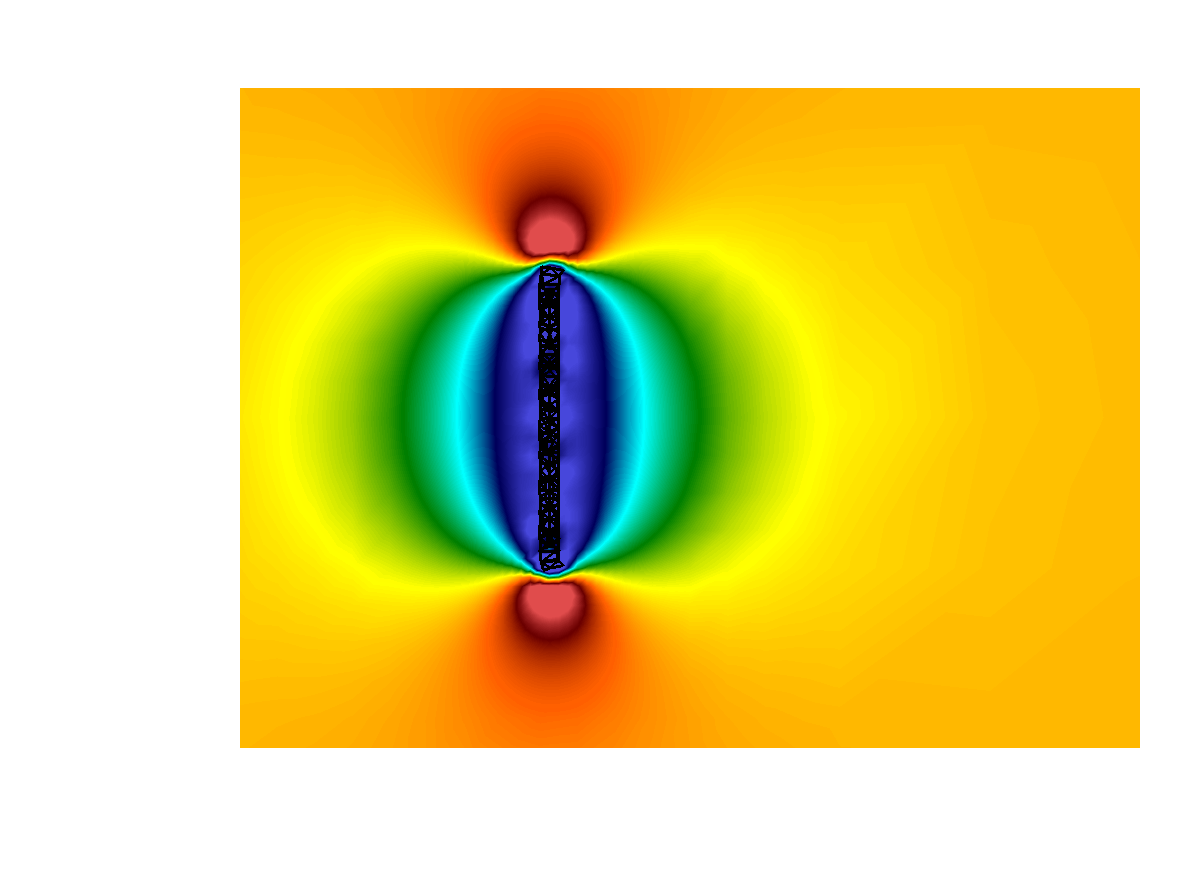
\includegraphics[width=\textwidth]{ch22-ux-slice-zoom-t05.png}\\
\scriptsize the fluid slice with the plate's section (chapter 22)
\end{columns}
\footnotesize
\begin{itemize}
  \item The 3D file (\code{viz\_IB3d/output.ex2}) lists \code{X\_0..X\_2}, \code{dX\_0..dX\_2}, \code{U\_0..U\_2}, \code{F\_0..F\_2}, \code{coordx..coordz}; VisIt 3.5 does \emph{not} build \code{dX}, \code{U}, \code{F}, \code{X} for this file (its expression list has only \code{mesh\_quality} and \code{time\_derivative} entries), while it does for the 2D files: in 3D the vector expression \code{\{dX\_0, dX\_1, dX\_2\}} is yours to define, exactly as in 2013.
\end{itemize}
\end{frame}

% 26b
\begin{frame}{Three dimensions: inside the mesh}
\label{fr:threed2}
\footnotesize
\begin{itemize}
  \item The Mesh plot of a volume mesh shows its outer surface; to see inside, \gui{Operators $\to$ Selection $\to$ Threshold} or \gui{Clip}, or a Slice through the mesh (which cuts the displaced mesh when the Displace operator comes first in the operator list: order matters, top of the list is applied first).
  \item The Displace operator accepts a 2-component \code{dX} in 3D without a word and displaces in $x$ and $y$ only (checked: the same $x$ and $y$ extents as with three components, $z$ unchanged): the picture looks almost right and the error is easy to miss, so define \code{\{dX\_0, dX\_1, dX\_2\}}.
  \item A Pseudocolor of a nodal field on a volume mesh colours the surface by the surface nodes' values; a Threshold on \code{mesh\_quality/aspect\_gamma} $> 4$ keeps the $337$ slivers alone and shows where the mesher put them (the plate's edges and corners).
  \item Chapter 22 read the two-material plate's two displacements from this file; chapter 27 has the cameras, slices and isosurfaces that make such pictures, chapter 18 the element-size rules and chapter 22's sliver slide the shape rules the \code{mesh\_quality} expressions check.
\end{itemize}
\end{frame}


% 27
\begin{frame}[fragile]{Export: the mesh with its fields as VTK}
\label{fr:export}
\footnotesize
\begin{columns}[T]
\column{0.5\textwidth}
\begin{lstlisting}[style=pytiny]
# File > Export database, or in the CLI:
e = ExportDBAttributes()
e.db_type = "VTK"; e.db_type_fullname = "VTK_1.0"
e.dirname = "/root/work/ch28_export"
e.filename = "plate"; e.variables = ("dX_0",)   # the call that wrote the file below
e.allTimes = 1; ExportDatabase(e)               # every state ... each overwriting the last (see right)
# one state: e.allTimes = 0; SetTimeSliderState(10); e.filename = "plate_0010"; ExportDatabase(e)
\end{lstlisting}
\begin{lstlisting}[style=tiny]
# what VisIt 3.5.0 wrote (headless): the file name is dropped, the file is <current directory>/.vtk
# vtk DataFile Version 4.2            # legacy ASCII, one time state
DATASET UNSTRUCTURED_GRID
FIELD FieldData 4                     # avtOriginalBounds, MeshName, CYCLE 0, TIME 4 (the last state)
POINTS 101 double                     # the reference positions (no Displace on the plot)
CELLS 130 520                         # the triangles
POINT_DATA 101
FIELD FieldData 1
dX_0 1 101 double                     # one array per exported variable (one asked for here)
\end{lstlisting}
\column{0.48\textwidth}
\scriptsize
\begin{itemize}
  \item With the Mesh plot selected (``highlight the mesh''), \gui{File $\to$ Export Database}: file name, directory, \gui{Export to: VTK}, \gui{Export all time states}, \gui{Add variable} for each field to carry (the mesh goes anyway), \gui{Apply}, then \gui{Export}. The export writes the mesh \emph{as plotted}: with the Displace operator on the active plot, the VTK points are the current positions; without it, the reference ones plus \code{dX}.
  \item Observed in 3.5.0 run headless: the \code{filename} and the directory are ignored and every call writes \code{.vtk} into the \emph{current directory} of the VisIt process (chapter 33 found this; chapter 28's test ran inside the export folder, where the two coincide), so \gui{Export all time states} overwrites itself; export one state at a time and rename the file (\code{os.rename}) after each call. The export options (\code{GetExportOptions('VTK')}) choose legacy or XML, ASCII or binary.
\end{itemize}
\end{columns}
\end{frame}

% 27b
\begin{frame}{Export: when and what for}
\label{fr:export2}
\begin{columns}[T]
\column{0.4\textwidth}
\begin{center}
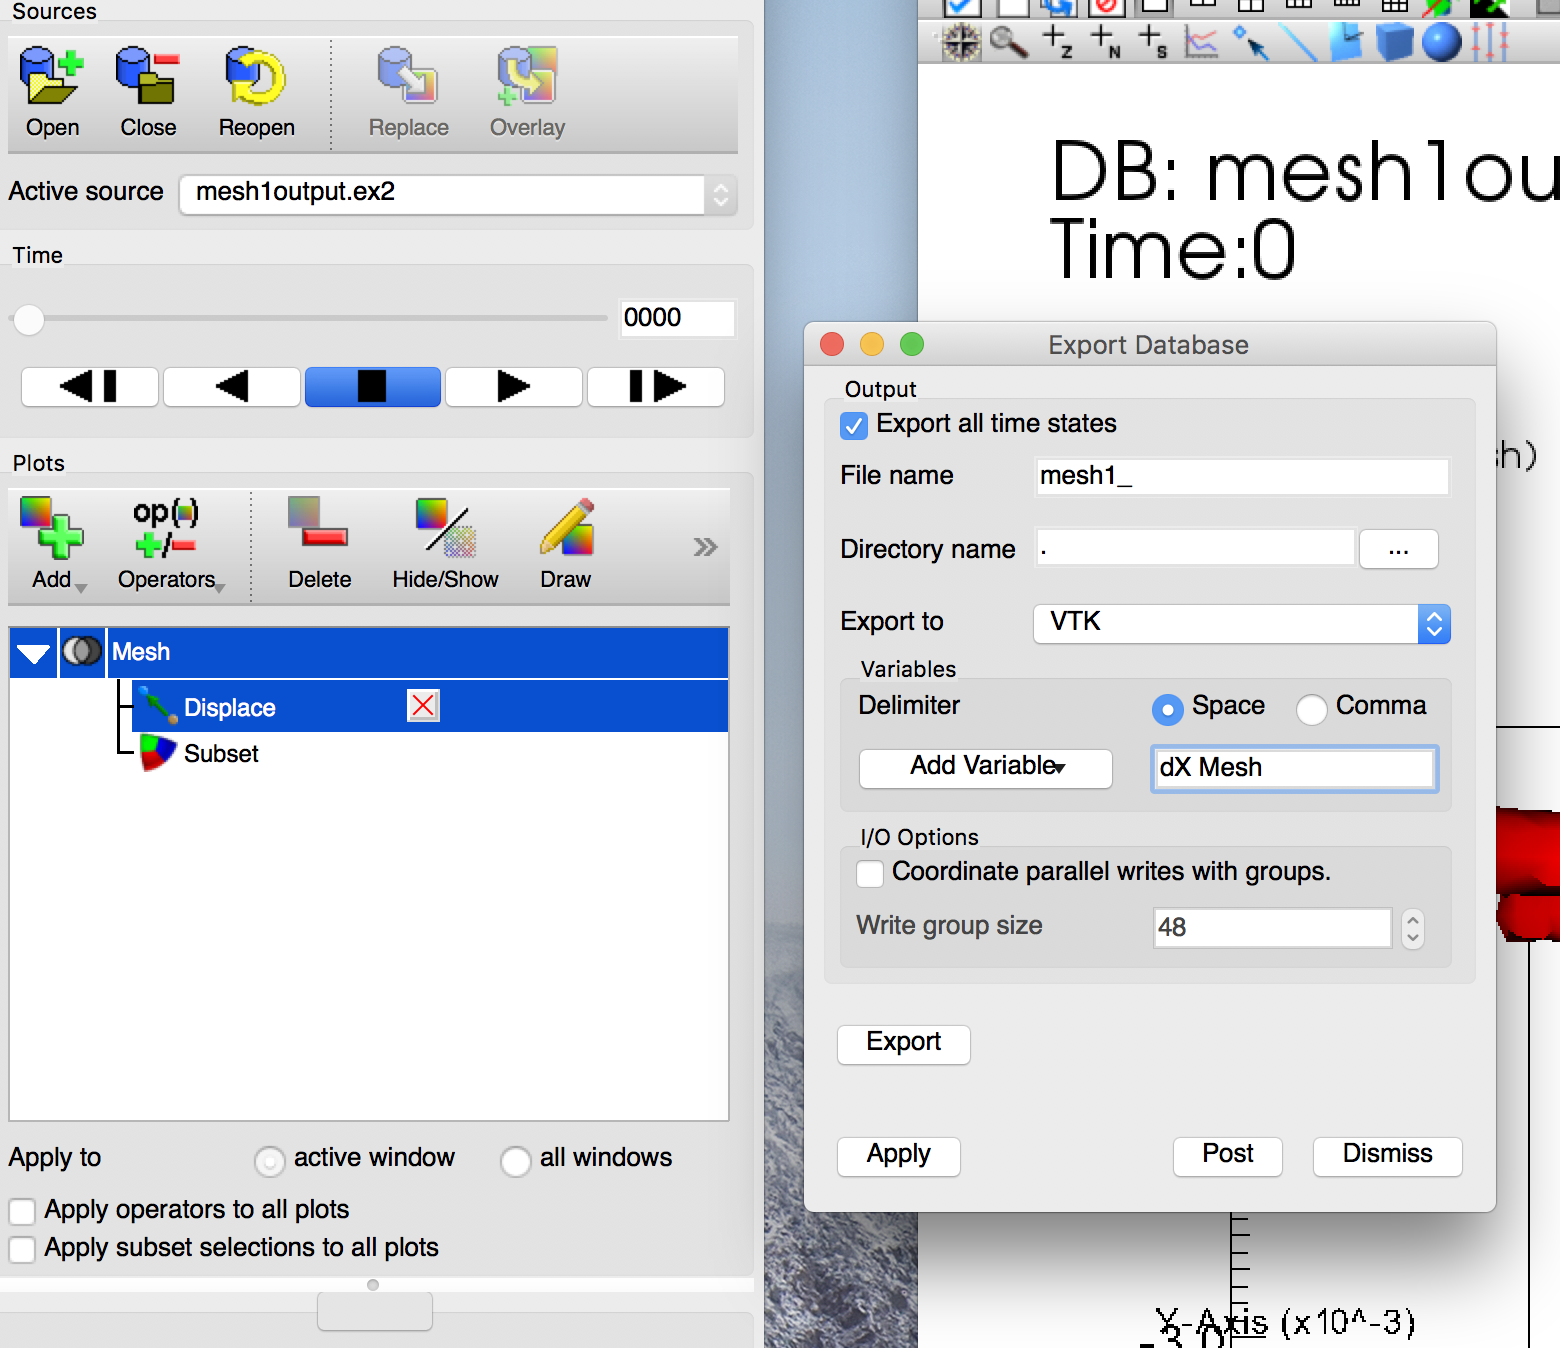
\includegraphics[width=0.95\textwidth]{ch28-l18-export.png}
\end{center}
\sourcecredit{Window: ``3B -- Analyzing your IBFE simulation'' (2018), VisIt 2.12.2.}
\column{0.58\textwidth}
\scriptsize
\begin{itemize}
  \item The 2018 reason: KillDevil's VisIt 2.12.3 had no Exodus reader, so the \code{.ex2} files were exported on a laptop and the VTK files read on the cluster (slide \ref{fr:recipe18}); ``if you are doing the standard fiber-based IBAMR, you do not need to worry about this step'' (a Silo run never needed it). VisIt 3.5 reads Exodus everywhere; the export is still the shortest way to an \code{.ex2} mesh in Python or MATLAB without netCDF (chapter 33: \code{pyvista} or the \code{vtk} module read the exported file in one line; \code{meshio} 5.3 cannot, because of the \code{FIELD} block VisIt writes).
  \item The 3.5 window is titled \gui{Export Database}; its button is \gui{Add variable}. Other export formats in the menu: Silo, Tecplot, Xmdv (columns of numbers), PLY and STL for the surface of a 3D mesh (a 3D-printable file of a deformed body, with the Displace operator on); the Silo points of a point-method run export the same way (a VTK polydata of points).
  \item The export takes the active plot's data after its operators: a Box or Threshold before the export writes the selected part only, and a Slice of a 3D mesh writes the cut surface.
\end{itemize}
\end{columns}
\end{frame}


% 28
\begin{frame}[fragile]{The \code{.curve} file: a time query out, into MATLAB or Python}
\label{fr:curve}
\footnotesize
\begin{columns}[T]
\column{0.5\textwidth}
\begin{lstlisting}[style=tiny]
# window 2 active; File > Set save options: file type Curve; Save
# (CLI: SaveWindowAttributes().format = s.CURVE)
# Max_dX_mag
0 0
0.1000000000000001 0.05183466718831264
0.2000000000000001 0.1011884718693308
0.3000000000000002 0.1510825088362431
...
# Average_Value_dX_mag
0 0
...
\end{lstlisting}
\begin{lstlisting}[style=tiny]
% MATLAB (2018 deck, slide 16; a block per curve in the file)
C = importdata('plate_dX_queries.curve');
t = C.data(:,1);  y = C.data(:,2);  plot(t, y)
\end{lstlisting}
\begin{lstlisting}[style=pytiny]
# Python: one block per curve; '#' lines are the headers
import numpy as np
blocks, cur = {}, None
for line in open("plate_dX_queries.curve"):
    if line.startswith("#"): cur = line[1:].strip(); blocks[cur] = []
    else: blocks[cur].append([float(v) for v in line.split()])
t, ymax = np.array(blocks["Max_dX_mag"]).T        # the other block: "Average_Value_dX_mag"
\end{lstlisting}
\column{0.48\textwidth}
\scriptsize
\begin{itemize}
  \item A \code{.curve} file is text: a \code{\#} header line with the curve's name, then \code{time value} pairs, one block per curve in the window. The 2018 deck's \code{importdata} reads the first block; with two curves in one window, split on the headers as the Python lines do, or save each curve from its own window.
  \item The same file comes from a \gui{Do time curve} pick (slide \ref{fr:pick}) and from a Lineout (chapter 29).
  \item \gui{Set save options} also offers \gui{ULTRA} (another text curve format) and \gui{VTK}; keep \code{.curve} for anything a script will read.
  \item Chapter 33 collects every way out: this file, the VTK export, the \code{hier\_data} text, netCDF for \code{.ex2} directly, HDF5 for the fluid dumps.
\end{itemize}
\end{columns}
\end{frame}

% 29
\begin{frame}{The 2018 recipe: analysing an IBFE run away from the GUI}
\label{fr:recipe18}
\begin{columns}[T]
\column{0.3\textwidth}\centering
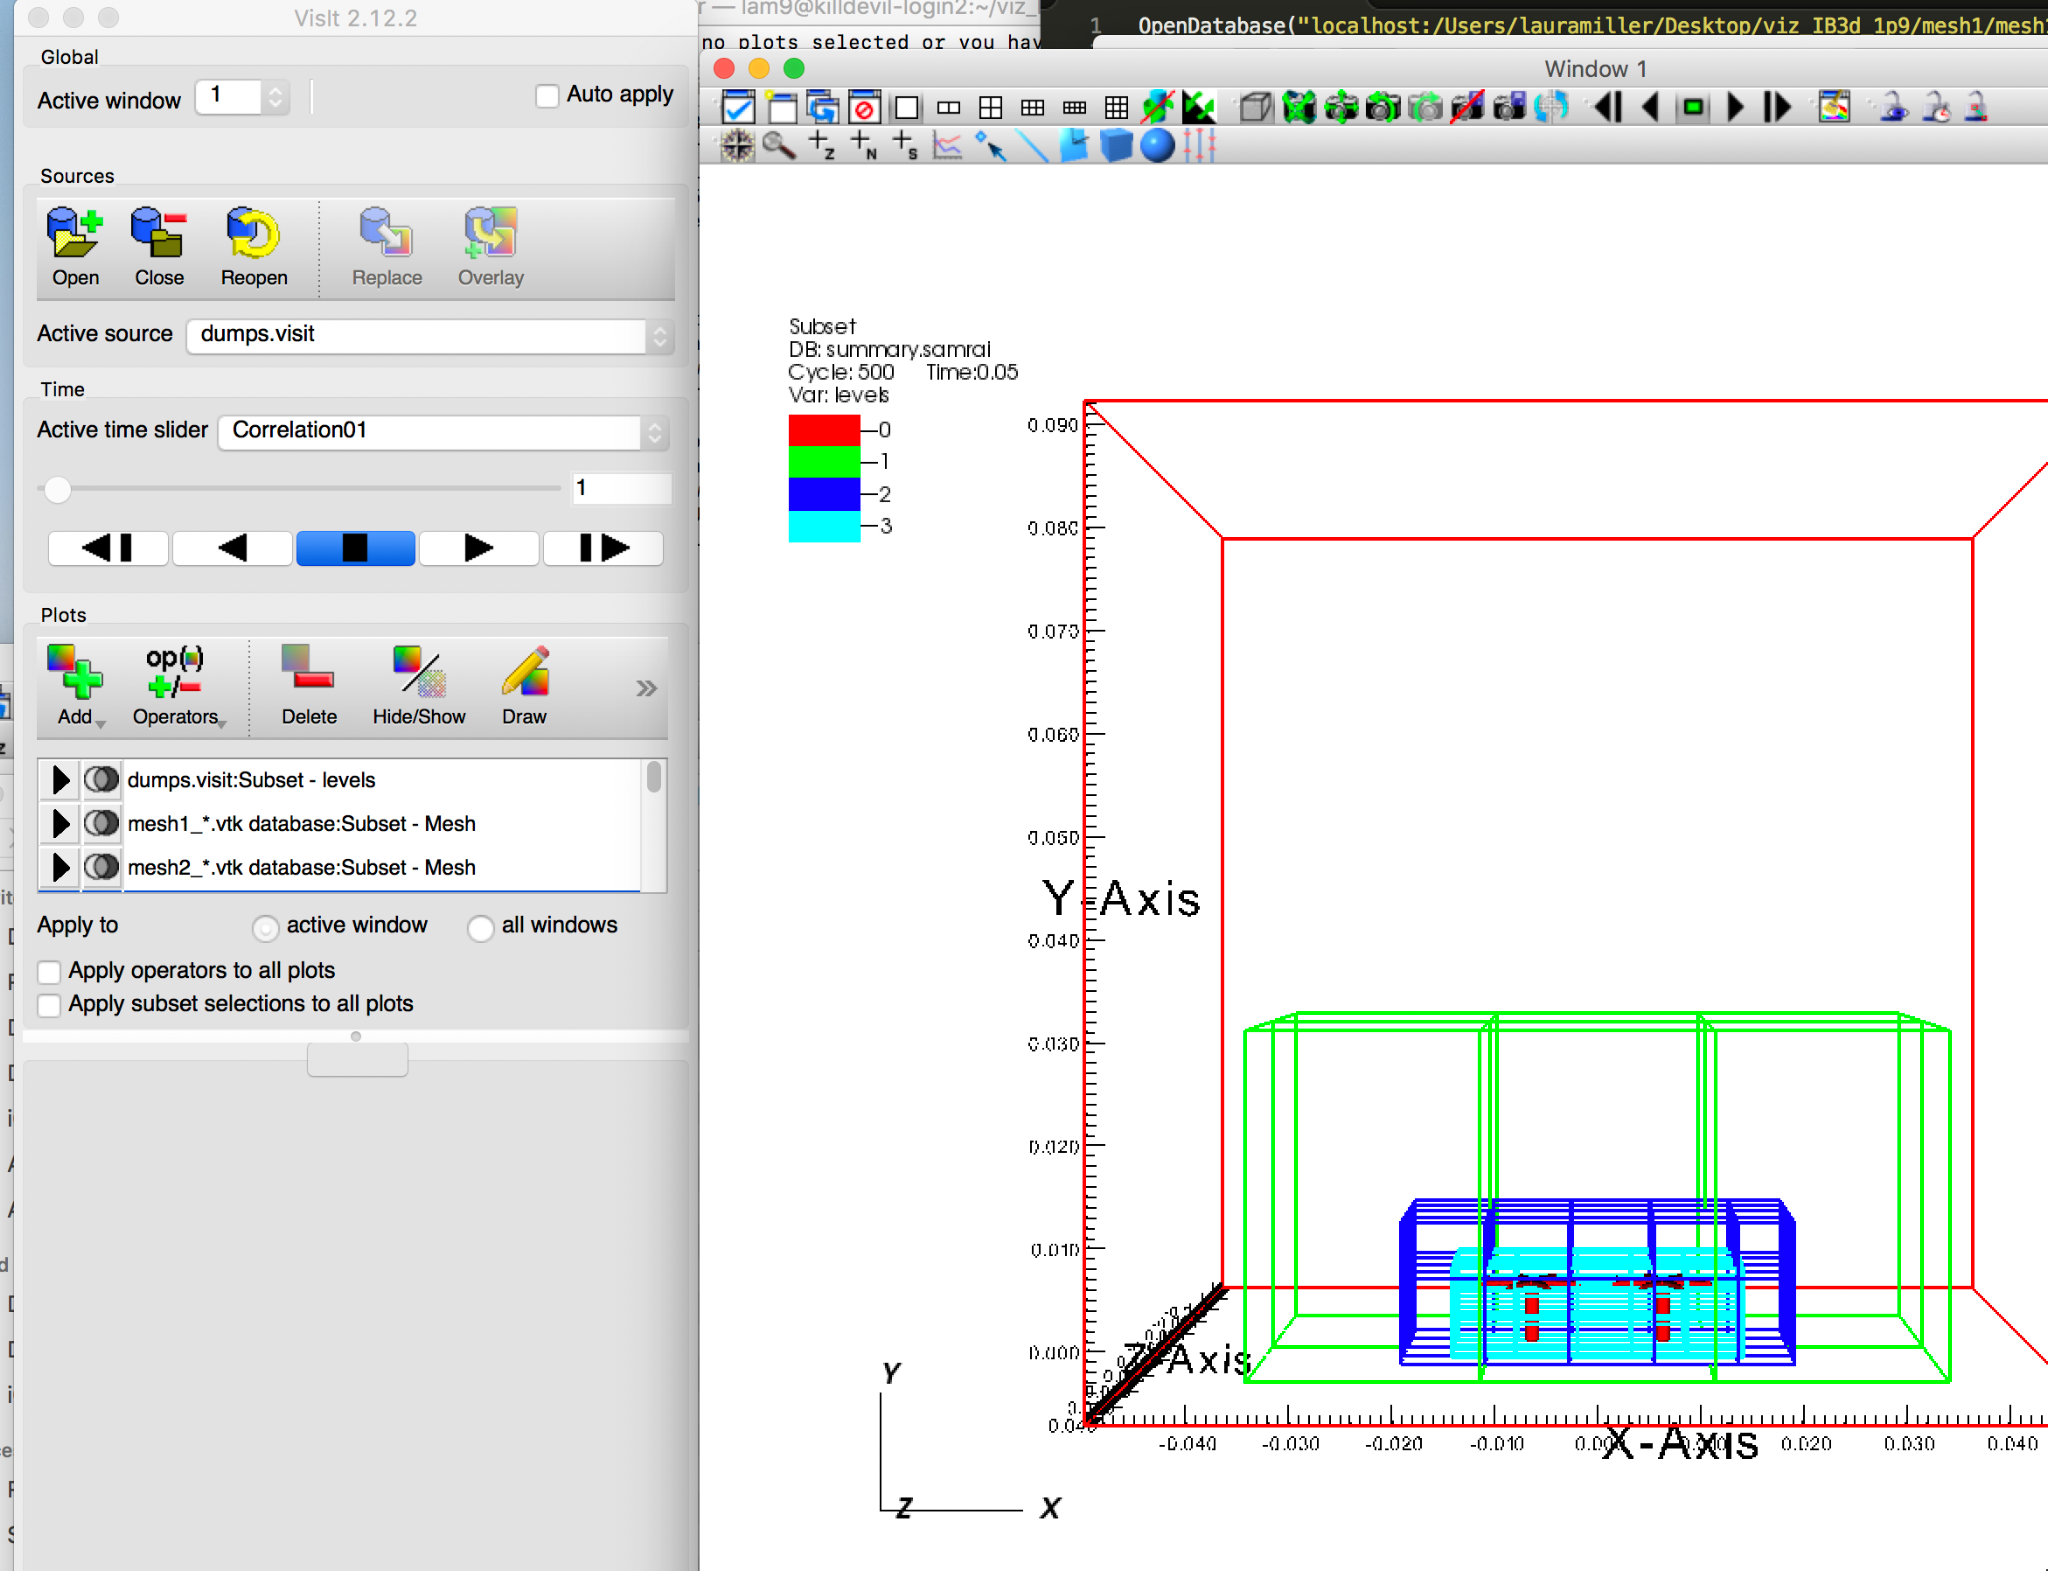
\includegraphics[width=0.95\textwidth]{ch28-l18-vtk-subsets.png}\\
\scriptsize two exported parts (\code{mesh1\_*.vtk}, \code{mesh2\_*.vtk}) as Subset plots with the fluid
\column{0.3\textwidth}\centering
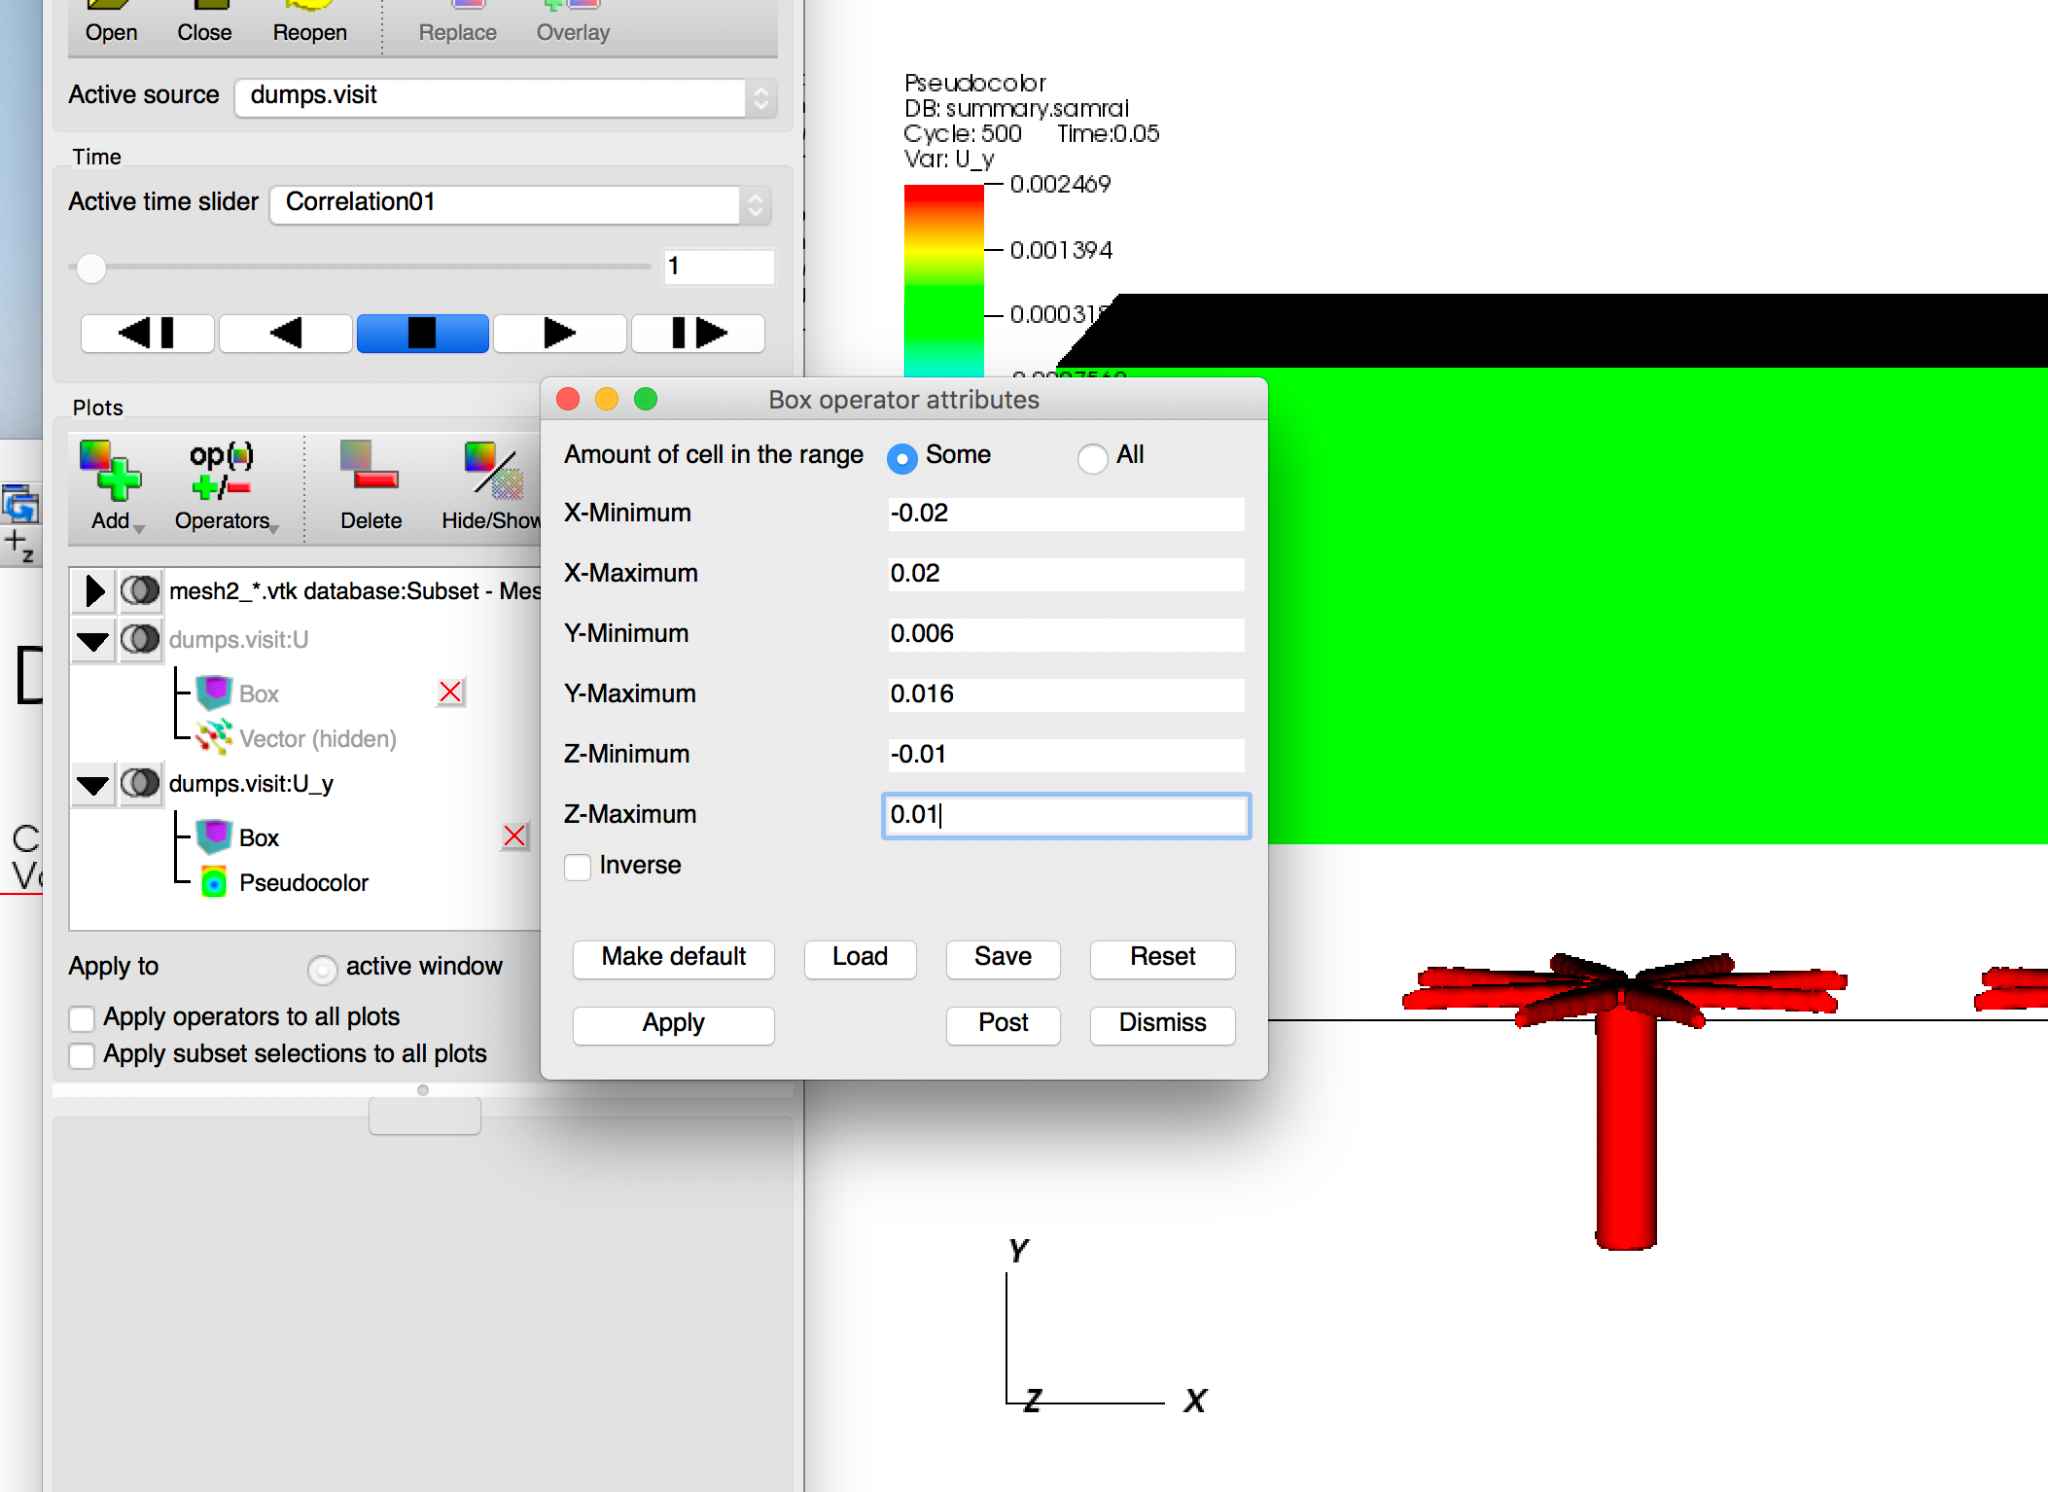
\includegraphics[width=0.95\textwidth]{ch28-l18-box.png}\\
\scriptsize the Box operator attributes: a box above the structures
\column{0.3\textwidth}\centering
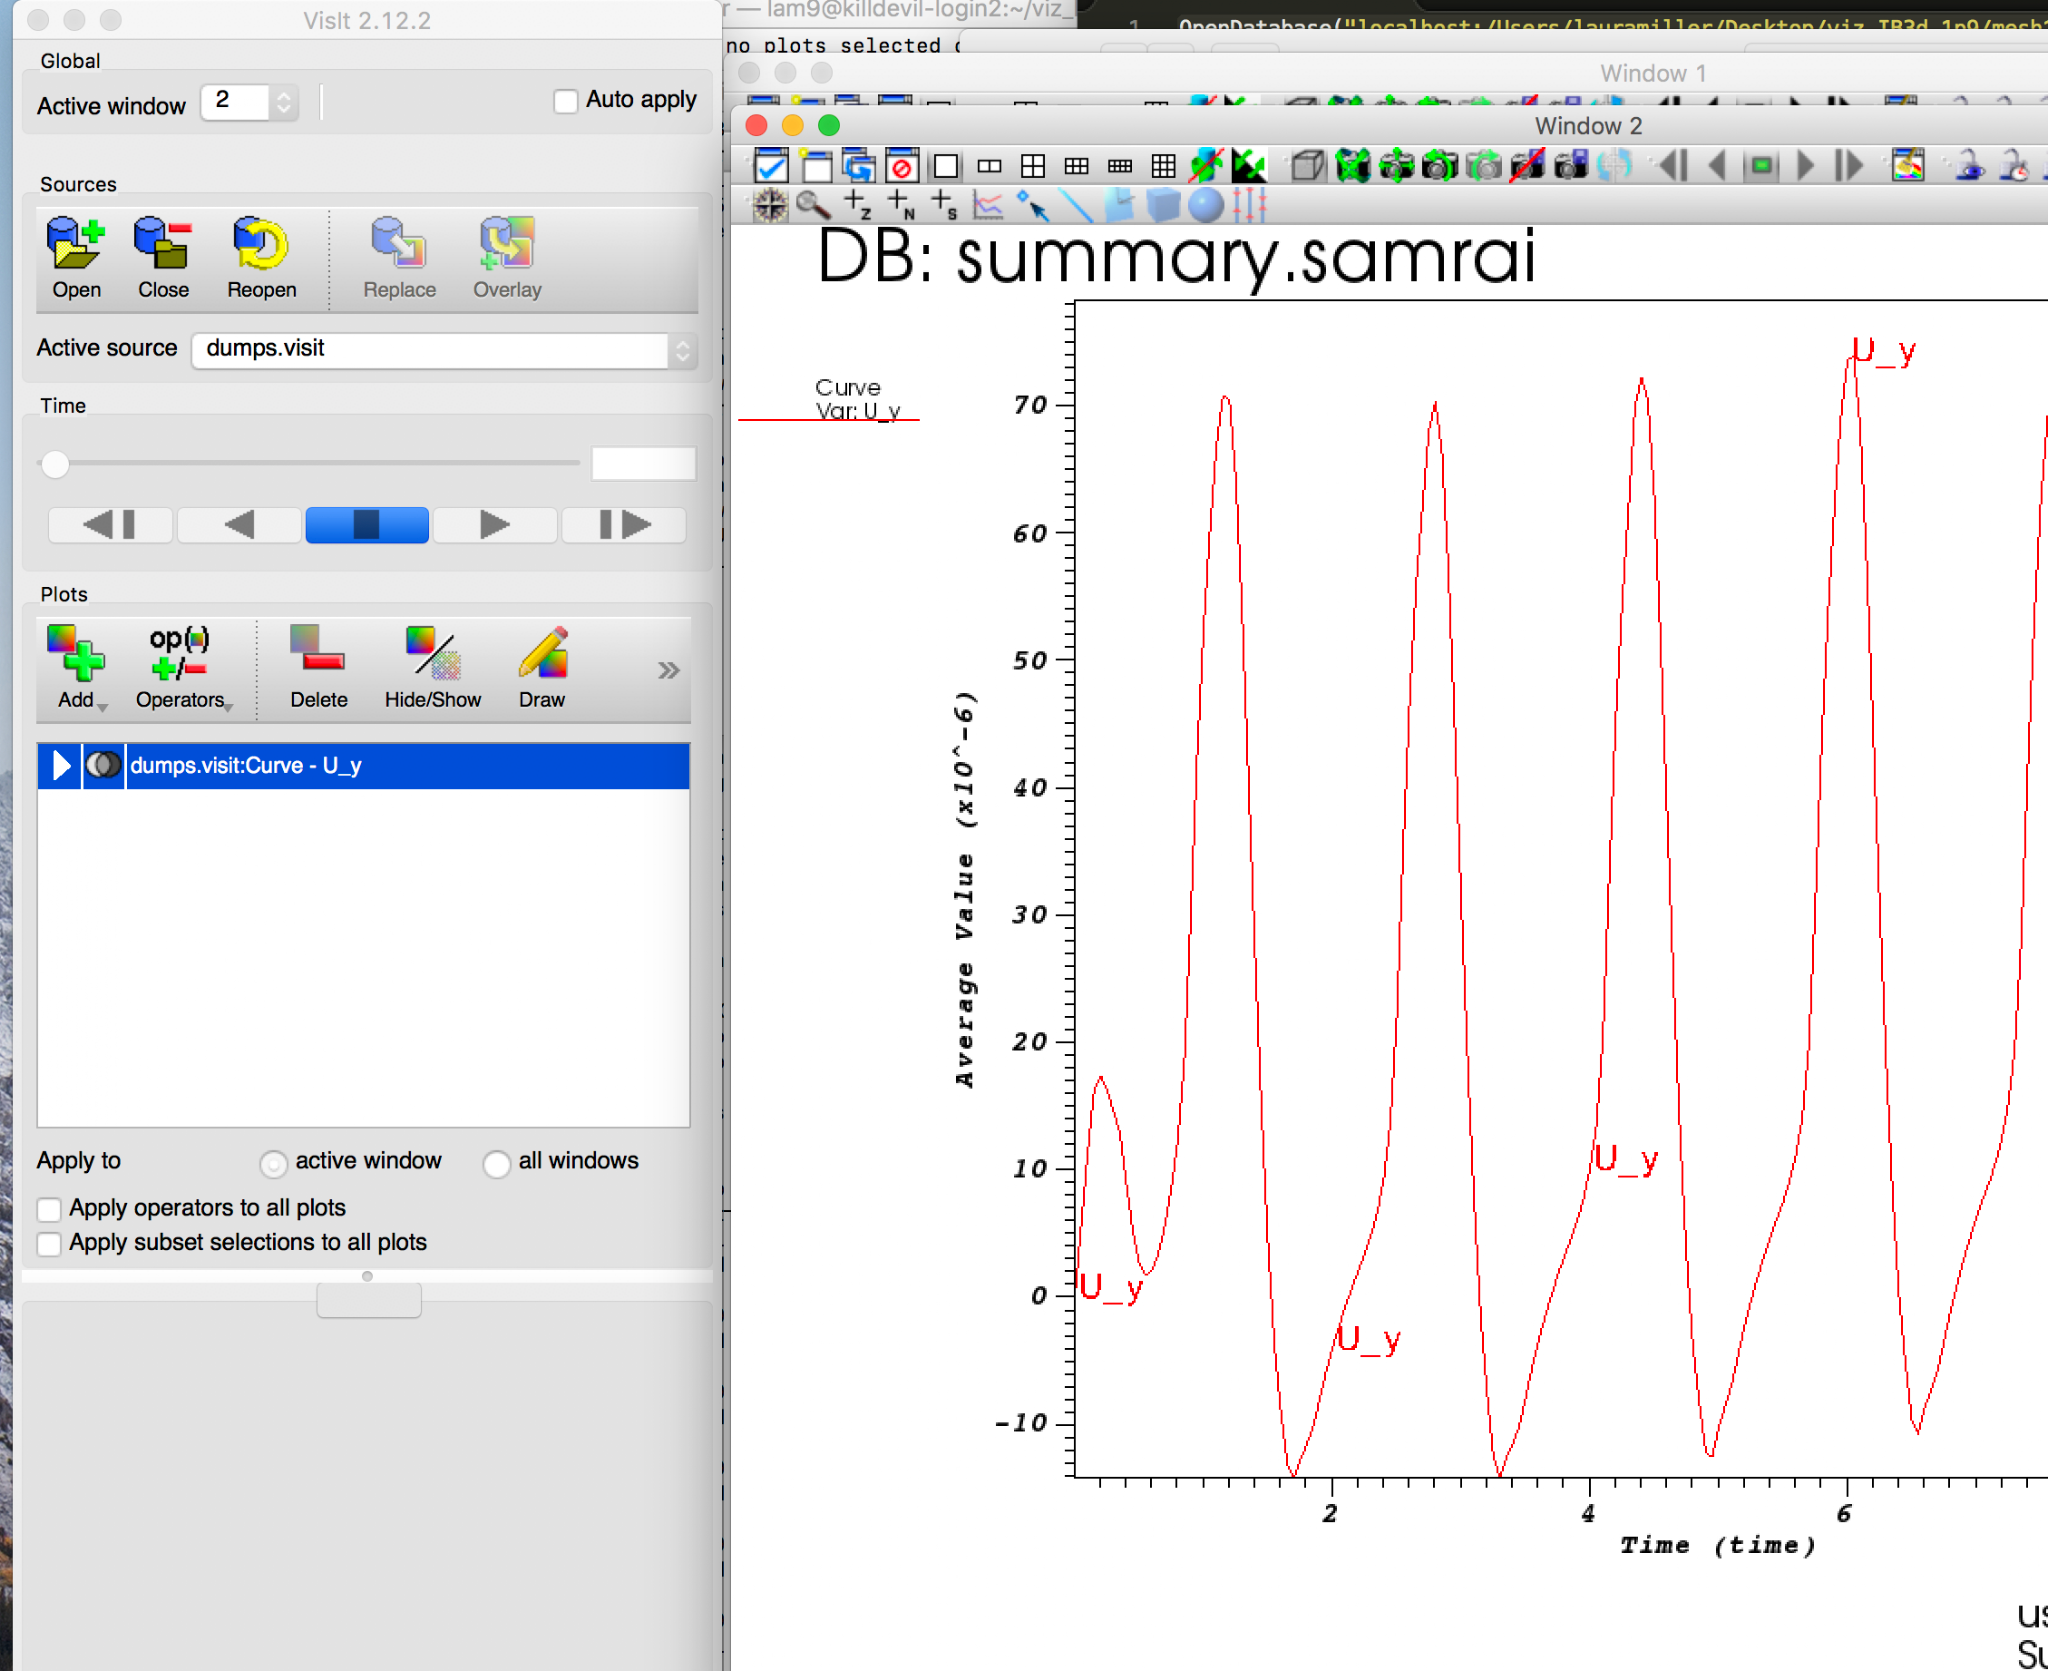
\includegraphics[width=0.95\textwidth]{ch28-l18-curve.png}\\
\scriptsize the averaged \code{U\_y} against time in window 2
\end{columns}
\footnotesize
\begin{enumerate}
  \item Open the \code{.ex2} files on the laptop, plot the mesh, displace it, \gui{File $\to$ Export database}, all time states, VTK, variables \code{dX} and Mesh (slide \ref{fr:export}).
  \item Close VisIt, reopen, start recording (chapter 32), open \code{dumps.visit} and the VTK files (\code{mesh1\_*.vtk database}), untick ``apply to all''.
\end{enumerate}
\sourcecredit{``3B -- Analyzing your IBFE simulation'' (MATH 769, 2018), VisIt 2.12.2 on a Mac and 2.12.3 on KillDevil.}
\end{frame}

% 29b
\begin{frame}{The 2018 recipe (2): the query, the file, the cluster}
\label{fr:recipe18b}
\footnotesize
\begin{enumerate}
  \setcounter{enumi}{2}
  \item Pseudocolor of \code{U\_y}; \gui{Operators $\to$ Selection $\to$ Box} around the region of interest (``of whatever size you like'', all three ranges, kept the same from run to run: ``what you pick does not matter too much as long as it's consistent''); \gui{Controls $\to$ Query over time options}, x-axis time; \gui{Query $\to$ Average Value}, \gui{Do Time Query}.
  \item Window 2 active; \gui{File $\to$ Set save options}, file type \code{curve}, \gui{Save}; stop recording; search the Python for every path and change it to the cluster's; run \code{visit -cli -nowin -s script.py} there.
\end{enumerate}
\begin{itemize}
  \item The run in the deck was a 3D two-coral case (\code{viz\_IB3d}); the pictures on the previous slide are its screenshots, kept as the record of the recipe.
  \item Steps 2 and 4's recording is chapter 32; step 3's Eulerian average is chapter 29; chapter 31 has the cluster side (modules, batch VisIt). The deck's own reading of the \code{.curve} file (``time is the first column, velocity is the second'') is right; the x-axis option is \code{DTime} in 3.x.
  \item What has changed: the cluster's VisIt reads Exodus now, so step 1 is optional; the paths are still the thing to search for (``I recommend doing a search to find all paths''); the \code{.curve} import into MATLAB is unchanged (slide \ref{fr:curve}).
\end{itemize}
\end{frame}


% 29c
\begin{frame}[fragile]{The 2018 recipe (3): the recorded script}
\label{fr:recipe18c}
\footnotesize
\begin{lstlisting}[style=pytiny]
# the deck's slide 15, as recorded on the Mac (VisIt 2.12.2): three databases, two exported parts as Subset plots
OpenDatabase("localhost:/Users/lauramiller/Desktop/viz_IB3d_1p9/mesh1/mesh1_*.vtk database", 0)
OpenDatabase("localhost:/Users/lauramiller/Desktop/viz_IB3d_1p9/mesh2/mesh2_*.vtk database", 0)
OpenDatabase("localhost:/Users/lauramiller/Desktop/viz_IB3d_1p9/dumps.visit", 0)
ActivateDatabase("localhost:/Users/lauramiller/Desktop/viz_IB3d_1p9/mesh1/mesh1_*.vtk database")
AddPlot("Subset", "Mesh", 1, 0)
ActivateDatabase("localhost:/Users/lauramiller/Desktop/viz_IB3d_1p9/mesh2/mesh2_*.vtk database")
AddPlot("Subset", "Mesh", 1, 0)
DrawPlots()
SubsetAtts = SubsetAttributes()
SubsetAtts.colorType = SubsetAtts.ColorByMultipleColors  # ColorBySingleColor, ColorByMultipleColors, ColorByColorTable
SubsetAtts.colorTableName = "Default"
SubsetAtts.invertColorTable = 0
SubsetAtts.filledFlag = 1
SubsetAtts.legendFlag = 0
SubsetAtts.lineStyle = SubsetAtts.SOLID  # SOLID, DASH, DOT, DOTDASH
\end{lstlisting}
\begin{itemize}
  \item ``In this code, there are paths throughout. Be sure to search and replace all'' (the Mac paths become the cluster's); ``stop recording, and cut and paste python commands to file''. A \code{*.vtk database} name opens a numbered series of VTK files as one time series. The recording itself, and the loop over states that saves a picture per frame (the deck's slide 7), are chapter 32.
\end{itemize}
\end{frame}

% 30
\begin{frame}[fragile]{Scripted: what made these pictures}
\label{fr:script}
\footnotesize
\begin{columns}[T]
\column{0.56\textwidth}
\begin{lstlisting}[style=pytiny]
viz = "/root/work/0.19.0/ibfe01_HALF/viz_IB2d"
OpenDatabase(viz + "/dumps.visit"); OpenDatabase(viz + "/output.ex2")
DefineScalarExpression("dX_mag", "magnitude(dX)")   # dX exists already
ActivateDatabase(viz + "/dumps.visit"); AddPlot("Pseudocolor", "Omega")
ActivateDatabase(viz + "/output.ex2")
AddPlot("Pseudocolor", "dX_mag")
AddOperator("Displace"); d = DisplaceAttributes(); d.variable = "dX"; d.factor = 1.0
SetOperatorOptions(d)                                 # on the active plot only
AddPlot("Mesh", "Mesh"); AddOperator("Displace"); SetOperatorOptions(d)
DrawPlots(); SetTimeSliderState(10)
PickByNode(0, 0, ("X_0", "X_1", "dX_1", "U_1", "F_1")); print(GetPickOutput())   # (node, domain): keyword form PickByNode(domain=0, element=k, vars=(...)) is safer
SetActivePlots(1); print(Query("Max"))               # the Pseudocolor plot
qt = GetQueryOverTimeAttributes(); qt.timeType = qt.DTime; SetQueryOverTimeAttributes(qt)
QueryOverTime("Max"); QueryOverTime("Average Value")  # -> window 2
AddOperator("Box"); b = BoxAttributes(); b.minx, b.maxx = 0.0, 1.0; SetOperatorOptions(b)
\end{lstlisting}
\column{0.42\textwidth}
\scriptsize
\begin{itemize}
  \item Every GUI step on these slides has a one-line CLI form, and the GUI's \gui{Controls $\to$ Command} window records them as you click (chapter 32, with the 2018 recording recipe).
  \item \code{AddOperator} and \code{SetOperatorOptions} act on the \emph{active} plot (\code{SetActivePlots}); passing \code{1} as a second argument applies to all plots, the scripted form of the checkbox.
  \item Queries need the right active plot: \code{Query("Max")} on a Mesh plot gives ``Cannot perform a Max query on variable Mesh''.
  \item The whole script of this chapter (\code{wsl/final/visit\_ch28.sh}) also exports the VTK and curve files and renders the 3D and Silo pictures; it runs headless (\code{visit -nowin -cli -s}).
\end{itemize}
\end{columns}
\end{frame}

% 31
\begin{frame}{Then and now}
\label{fr:thennow}
\scriptsize
\renewcommand{\arraystretch}{0.95}
\begin{tabular}{@{}L{0.42\textwidth}L{0.51\textwidth}@{}}
\toprule
the decks said (2013--2020) & VisIt 3.5 with IBAMR 0.19 \\
\midrule
``open \code{dump.visit}'' & the file is \code{dumps.visit} \\
create the vector expression \code{dX = \{dX\_0, dX\_1, 0\}}, save it as XML & VisIt builds \code{dX}, \code{U}, \code{F}, \code{X} from the components on opening; 2D files have two components; expressions you add are saved with the session \\
\gui{Operators $\to$ Transforms $\to$ Project} to flatten the 2D mesh & not needed: the mesh is two-dimensional \\
``\code{vist\_dump.xxxxx}: stores all the Cartesian grid data from each core'' & \code{visit\_dump.NNNNN}, listed by \code{dumps.visit} \\
x-axis ``Time'' in the query-over-time options & \gui{Time} in the window, \code{DTime} in the attributes (\gui{Cycle}, \gui{Timestep} the others) \\
``\gui{Control $\to$ Annotations}'' & \gui{Controls $\to$ Annotation} \\
``velocity exerted on the mesh'' & the mesh's velocity \code{U}, interpolated from the fluid \\
``\code{sqrt(dX\_0*dX\_0 + dX\_1*dX\_1)} gives the radial component'' & the in-plane displacement magnitude; the radial part is a projection (slide \ref{fr:expr}) \\
the cluster's VisIt cannot read \code{.ex2}: export as VTK first & the Exodus reader ships in every standard VisIt binary (a cluster's own build may omit it: check \gui{File $\to$ File information} there); export when a script wants VTK \\
``ex2: Cavity flow with mesh at bottom / ex3: Cavity flow with mesh at bottom / ex6: Flow past beam and block'' & chapter 25's table: ex2 is a soft plate pushed by a traction difference, ex3 a soft block under a sliding lid, ex6 the Turek--Hron beam (the shell test is ex1); slide \ref{fr:list2013} \\
Python 2 CLI, \code{module add visit/2.12.3} & Python 3 inside VisIt 3.x; chapter 31 for the cluster modules \\
\bottomrule
\end{tabular}
\end{frame}

% 31b
\begin{frame}{The 2013 examples list, and what the examples are}
\label{fr:list2013}
\scriptsize
\begin{tabular}{@{}L{0.33\textwidth}L{0.6\textwidth}@{}}
\toprule
the 2013 document's ``Examples List'' & chapter 25's description of the same upstream IBFE example \\
\midrule
``ex0: Rubber band'' & an elastic ring at rest in a periodic box with the exact pressure jump set: a static equilibrium test \\
``ex1: Stretched rubber band'' & the same ring started as an ellipse: the dynamic shell test of Griffith and Luo \\
``ex2: Cavity flow with mesh at bottom'' & a soft plate across a $2\times1$ box pushed by a traction difference, no tether \\
``ex3: Cavity flow with mesh at bottom'' & a soft block on the floor of a lid-driven cavity: a solid deformed by a shear flow \\
``ex4: Cavity flow with deformable ball'' & a soft disc in a lid-driven cavity (Griffith and Luo's Fig.\ 10) \\
``ex5: Flow past cylinder'' & a cylinder at $\mathrm{Re} = 200$: vortex shedding, $C_D$ and $C_L$; aborts as shipped (chapter 25) \\
``ex6: Flow past beam and block (square with long rectangular tail)'' & a rigid disc with an elastic beam behind it in a channel: the Turek--Hron FSI3 benchmark \\
\bottomrule
\end{tabular}

\begin{itemize}
  \item The 2013 document's note ``Can have multiple files of this type for different parts of object (see ex6)'' is right: ex6 writes one Exodus file per part (slide \ref{fr:parts}). Its two identical lines for ex2 and ex3 are the copy error chapter 25 corrected; the examples after ex6 (ex7--ex11) came later.
\end{itemize}
\end{frame}

% 32
\begin{frame}{What can go wrong (1)}
\label{fr:wrong}
\scriptsize
\renewcommand{\arraystretch}{0.95}
\begin{tabular}{@{}L{0.36\textwidth}L{0.57\textwidth}@{}}
\toprule
symptom & cause and fix \\
\midrule
``An invalid variable (dX) was specified'' and an empty window & \gui{Apply operators to all plots} was ticked: the fluid plot got the Displace operator; remove it from that plot and untick \\
the mesh sits where it started while the fluid moves & no Displace operator on that plot, or its variable is \gui{default}; every plot that should move needs its own \\
the mesh is drawn as a copy shifted by its reference coordinates & the Displace variable is \code{X} (the position) instead of \code{dX}: VisIt draws $\mathbf{s} + \mathbf{X}$ instead of $\mathbf{s} + \mathbf{dX}$ \\
in 3D the mesh moves in $x$ and $y$ but not in $z$ & a 2-component \code{dX}, accepted silently: use \code{\{dX\_0, dX\_1, dX\_2\}}, which 3.5 does not define for you in 3D \\
``Cannot perform a Max query on variable Mesh'' & queries need the Pseudocolor (or Vector) plot active, not the Mesh plot \\
``An invalid variable (\code{<name>\_mesh}) was specified'' & the structure has no springs, so no \code{\_mesh} was registered: draw \code{<name>\_vertices} \\
no \code{output.ex2} in \code{viz\_IB2d} & \code{viz\_dump\_interval = 0} (no dumps at all), or the program never reached its first dump; the \code{"ExodusII"} word in \code{viz\_writer} is not the switch (slide \ref{fr:exodus}) \\
no \code{lag\_data.visit} & \code{viz\_writer} lacks \code{"Silo"} (and an IB/01-style program crashes at the first dump) \\
\bottomrule
\end{tabular}
\end{frame}

% 32b
\begin{frame}{What can go wrong (2)}
\label{fr:wrong2}
\scriptsize
\renewcommand{\arraystretch}{0.9}
\begin{tabular}{@{}L{0.36\textwidth}L{0.57\textwidth}@{}}
\toprule
symptom & cause and fix \\
\midrule
\code{lag\_data.visit} has only positions & by design: forces and velocities of a point-method run are in \code{hier\_data} (chapter 11); the displacement is a cross-time expression (slide \ref{fr:cmfe}) \\
new states do not appear while a run is going & VisIt read the file once: \gui{File $\to$ ReOpen} (the Exodus file grows in place; the \code{.visit} lists grow by lines) \\
after a restart the plate file starts over at state 1 & the program did not call \code{append(from\_restart)}; the old states are gone (rerun from the restart with it, or keep the first file's copy) \\
the fluid and the mesh are out of step & different dump intervals or a declined correlation: \gui{Controls $\to$ Database correlations} \\
a Subset or Threshold leaves nothing & \gui{Threshold}'s \gui{Show zone if: Part in range / All in range} (\code{zonePortions}) or an empty box; check the ranges against \gui{SpatialExtents} \\
a query returns nothing & the plot is hidden (a hidden plot cannot be queried), or the Mesh plot is the active one \\
the Box keeps the wrong part & operator order: Displace before Box selects by current position, after it by reference position \\
a Pseudocolor of the mesh looks blocky in 3D & only the outer faces are drawn; Clip or Threshold to look inside \\
the exported VTK file is called \code{.vtk}, in the wrong folder & 3.5.0 headless drops the file name and the directory (it writes into VisIt's current directory); rename after each export (slide \ref{fr:export}; chapter 33's \code{resample\_export.py} does it) \\
\code{mesh\_quality/aspect} is zero everywhere & it is not defined for triangles in 3.5; use \code{minimum\_angle}, \code{condition} or \code{shape} in 2D, \code{aspect\_gamma}, \code{condition} or \code{shape} in 3D \\
\bottomrule
\end{tabular}
\end{frame}


% 33
\begin{frame}{Exercises}
\label{fr:exercises}
\footnotesize
\begin{enumerate}
  \item Run IBFE/01 with \code{MOTION = "ROTATE"} and draw the plate at $t = 1$, $2$ and $4$ over the vorticity, coloured by \code{magnitude(U)}; which end moves fastest after the release?
  \item Pick the two tips (the nodes at $x = \pm 0.5$ on the centre line) with \gui{Do time curve} and reproduce the README's HALF numbers ($y = +0.5$ at $t = 1$, $-0.5$ at $t = 3$ for the tethered tip; the lag of the free one).
  \item Query the average of \code{magnitude(F)} over the free half (Box, $x < 0$) and over the tethered half against time; where does the tether work hardest?
  \item On IBFE/08 (two files): draw the beam coloured by \code{dX\_1} and the circle by \code{magnitude(U)}, each displaced; then colour both by \code{ElementBlock} and explain the legend.
  \item On IB/13: build the cross-time displacement of slide \ref{fr:cmfe} and query its maximum over the cycle; compare with the drift chapter 9a's figures measured from the \code{X.*} files.
  \item Export IBFE/01's plate at $t = 1$ to VTK with \code{dX} and \code{F}, and read the file back in Python (chapter 33's reader, or \code{meshio}); check the tip's \code{dX\_1} against the Pick output.
  \item Threshold the 3D plate of IBFE/10 on \code{mesh\_quality/aspect\_gamma} above its 99th percentile and count the elements; where are they (chapter 22's sliver note)?
  \item Replace step 5 of slide \ref{fr:recipe} by the Project operator on purpose: does anything change? Then set the Displace multiplier to 10 and say what the picture now shows.
\end{enumerate}
\end{frame}

% 34
\begin{frame}{Rules of thumb}
\label{fr:thumb}
\small
\begin{itemize}
  \item Points: \code{lag\_data.visit} has positions only; the numbers live in \code{hier\_data}. Elements: \code{output.ex2} has everything, one file per part.
  \item Untick \gui{Apply operators to all plots} before anything else; then Displace with \code{dX}, one operator per plot that moves.
  \item Colour the structure by its own fields (\code{dX}, \code{U}, \code{F} and expressions); draw the Mesh plot on top with opaque mode off.
  \item Pick for one node, query for a field, select before you query a part; put the selection on the plot you query.
  \item \code{mesh\_quality} at the reference state judges the mesher, at a later state the deformation.
  \item Export VTK for scripts, \code{.curve} for time series; save the session next to the figure.
\end{itemize}
\end{frame}

% 35
\begin{frame}{Summary}
\label{fr:summary}
\footnotesize
\begin{enumerate}
  \item A point-method run writes its structures to Silo (\code{lag\_data.visit}: \code{<name>\_vertices} as points, \code{<name>\_mesh} as spring edges, one file per rank but every structure in rank 0's, in Lagrangian order; no fields), an IBFE run to ExodusII (\code{output.ex2} per part: the reference mesh and the nodal \code{X}, \code{dX}, \code{U}, \code{F} at every dump).
  \item The finite-element mesh is drawn where it is by the Displace operator with \code{dX}, which VisIt 3.x already defines; the operator must sit on each plot that should move and must not reach the fluid's.
  \item The mesh's fields colour it (Pseudocolor), move with it (Vector) and judge it (\code{mesh\_quality}); expressions combine them; selections cut it down; Pick and the time queries turn it into numbers and curves.
  \item IB points have no \code{dX}, but a cross-time expression builds the displacement from the positions; the domain Subset has one domain per structure, not per rank.
  \item Exported VTK files and \code{.curve} text are the hand-over to Python and MATLAB (chapter 33) and the scripted versions of all of this are chapter 32.
\end{enumerate}
\begin{homebox}
\footnotesize Next: chapter 33, converting between data types and exporting to MATLAB and Python; then the IB2d chapters, then chapter 27 (3D), 29 (data analysis), 30 (movies), 31 (the cluster) and 32 (the command line).
\end{homebox}
\end{frame}

% 36
\begin{frame}{Recordings and screenshots}
\label{fr:videos}
\small
\begin{itemize}
  \item Shannon Jones's YouTube video on visualizing the finite-element mesh (\code{watch?v=Kj\_MACemSd0}), referenced by every re-issue of the 2013 recipe from 2018 on (the 2017 IBFE Read Me: ``The youtube tutorial by shannon has a mistake, but this is corrected in the google slides''); and her channel's six VisIt how-tos (the 2017 ``Visit Analysis and Python'' Read Me; chapter 32). Listed, not incorporated.
  \item The 2020 Zoom recording of IBFE Lecture 1 (\emph{BeamExample}, 20 May 2020), whose slides 18--26 are the 2020 form of this recipe, is in the front matter's list (chapter 0.1).
  \item The window screenshots here are the 2013, 2014 and 2018 decks' (VisIt 2.x, 2.7.2 and 2.12.2 on a Mac), credited on each slide; the re-shoot list in \code{plan/visit-screenshots-todo.md} now has a chapter 28 section (the Displace window with its Vectors submenu, the Pick window, the Query window with ``All queries-over-time'' and ``Do Time Query'', the Export database window, all in 3.5).
\end{itemize}
\end{frame}

% 37
\begin{frame}{References and credits}
\label{fr:refs}
\scriptsize
\begin{itemize}
  \item A. Hoover, \emph{IBAMR Finite Element Visualization with VisIt} (Miller Lab, 23 May 2013) and \emph{5-IBFE Tutorial: Visualizing Lagrangian Data} (2014); B. Griffith's description of the Exodus output (IBAMR users' list, quoted in the April 2013 MATH 769 deck); S. Jones's video how-tos; the 2018 MATH 769 deck \emph{3B -- Analyzing your IBFE simulation}.
  \item IBAMR 0.19.0 source: \code{ibtk/src/lagrangian/LSiloDataWriter.cpp} and \code{include/ibtk/LSiloDataWriter.h} (file names, \code{registerMarkerCloud}, \code{registerUnstructuredMesh}, \code{registerVariableData}); \code{src/IB/IBRedundantInitializer.cpp} (\code{initializeLSiloDataWriter}: the \code{\_vertices}, \code{\_mesh}, \code{\_xmesh}, \code{\_rod\_mesh} names); \code{src/IB/FEMechanicsBase.cpp} (the systems and their variables); \code{examples/IBFE/explicit/ex0/example.cpp} (\code{ExodusII\_IO}, \code{append}, \code{write\_timestep}). \url{https://github.com/IBAMR/IBAMR}.
  \item libMesh, \code{ExodusII\_IO} (\url{https://libmesh.github.io/doxygen/classlibMesh_1_1ExodusII__IO.html}); Silo (\url{https://silo.readthedocs.io/}); VisIt 3.5.0 (\url{https://visit-dav.github.io/visit-website/}) and its user manual's chapters on the Displace operator, expressions (\code{conn\_cmfe}, \code{pos\_cmfe}, \code{coords}), Pick, Query over time, the Selection operators, Export database and the Curve format.
  \item Data: this series' IBFE/01 (FULL and HALF), IBFE/08, IBFE/10, IB/13 and IB/08 runs and upstream IBFE ex7, IBAMR 0.19.0, four cores; pictures by \code{wsl/final/visit\_ch28.sh}; the exported VTK and curve files as shown.
\end{itemize}
\end{frame}

\end{document}
